% Sablon pentru realizarea lucrarii de licenta, conform cu recomandarile
% din ghidul de redactare:
% - https://fmi.unibuc.ro/finalizare-studii/
% - https://drive.google.com/file/d/1xj9kZZgTkcKMJkMLRuoYRgLQ1O8CX0mv/view

% Multumiri lui Gabriel Majeri, acest sablon a fost creat pe baza
% codului sursa a lucrarii sale de licenta. 
% Codul sursa: https://github.com/GabrielMajeri/bachelors-thesis
% Website: https://www.gabrielmajeri.ro/
%
% Aceast sablon este licentiat sub Creative Commons Attribution 4.0 International License.

\documentclass[12pt, a4paper]{report}

% Modificarea geometriei paginii
\usepackage{geometry}

% Suport pentru diacritice și alte simboluri
\usepackage{fontspec}

% Suport pentru mai multe limbi
\usepackage{polyglossia}

% Setează limba textului la română
\setdefaultlanguage{romanian}
% Am nevoie de engleză pentru rezumat
\setotherlanguages{english}

% Indentează și primul paragraf al fiecărei noi secțiuni
\SetLanguageKeys{romanian}{indentfirst=true}

% Suport pentru diferite stiluri de ghilimele
\usepackage{csquotes}

\DeclareQuoteStyle{romanian}
  {\quotedblbase}
  {\textquotedblright}
  {\guillemotleft}
  {\guillemotright}

% Utilizează biblatex pentru referințe bibliografice
\usepackage[
    maxbibnames=50,
    sorting=nty,
    backend=biber,
    style=numeric
]{biblatex}

\addbibresource{bibliography.bib}

% Setează spațiere inter-linie la 1.5
\usepackage{setspace}
\onehalfspacing

% Include funcțiile de grafică
\usepackage{graphicx}
% Încarcă imaginile din directorul `images`
\graphicspath{{./images/}}

% Listări de cod
\usepackage{listings}

% definirea culorilor
\usepackage{xcolor}

\definecolor{codeblue}{rgb}{0.11, 0.56, 1}
\definecolor{codegold}{rgb}{0.8, 0.64, 0}
\definecolor{codegray}{rgb}{0.3, 0.3, 0.3}
\definecolor{codepurple}{rgb}{0.7, 0.5, 0.7}

\lstdefinestyle{mystyle}{
    commentstyle=\color{codepurple},
    keywordstyle=\color{codeblue},
    numberstyle=\tiny\color{codegray},
    stringstyle=\color{codegold},
    basicstyle=\ttfamily\footnotesize,
    breakatwhitespace=false,         
    breaklines=true,                 
    captionpos=b,                    
    keepspaces=true,                 
    numbers=left,                    
    numbersep=5pt,                  
    showspaces=false,                
    showstringspaces=false,
    showtabs=false,                  
    tabsize=2
}

\lstset{style=mystyle}

% Linkuri interactive în PDF
\usepackage[
    colorlinks,
    linkcolor={black},
    menucolor={black},
    citecolor={black},
    urlcolor={blue}
]{hyperref}

% Simboluri matematice codificate Unicode
\usepackage[warnings-off={mathtools-colon,mathtools-overbracket}]{unicode-math}

% Comenzi matematice
\usepackage{amsmath}
\usepackage{mathtools}

% Formule matematice
\newcommand{\bigO}[1]{\symcal{O}\left(#1\right)}
\DeclarePairedDelimiter\abs{\lvert}{\rvert}

% Suport pentru rezumat în două limbi
% Bazat pe https://tex.stackexchange.com/a/70818
\newenvironment{abstractpage}
  {\cleardoublepage\vspace*{\fill}\thispagestyle{empty}}
  {\vfill\cleardoublepage}
\renewenvironment{abstract}[1]
  {\bigskip\selectlanguage{#1}%
   \begin{center}\bfseries\abstractname\end{center}}
  {\par\bigskip}

% Suport pentru anexe
\usepackage{appendix}

% Stiluri diferite de headere și footere
\usepackage{fancyhdr}

\fancypagestyle{front}{
  \fancyhf{}
  \renewcommand{\headrulewidth}{0pt}
  \cfoot{}
}
\fancypagestyle{main}{
  \fancyhf{}
  \renewcommand\headrulewidth{0pt}
  \fancyhead[C]{}
  \fancyfoot[C]{\thepage}
}

% Metadate
\title{Atacuri Speculative}
\author{Radu Ștefan-Octavian}

% Generează variabilele cu @
\makeatletter

\begin{document}

% Front matter
\cleardoublepage
\pagestyle{front}
\let\ps@plain\ps@front

% Pagina de titlu
\begin{titlepage}

% Redu marginile
\newgeometry{left=2cm,right=2cm,bottom=1cm}

\begin{figure}[!htb]
    \centering
    \begin{minipage}{0.2\textwidth}
        
\includegraphics[width=\linewidth]{logo-ub.png}
    \end{minipage}
    \begin{minipage}{0.5\textwidth}
        \large
        \vspace{0.2cm}
        \begin{center}
            \textbf{UNIVERSITATEA DIN BUCUREȘTI}
        \end{center}
        \vspace{0.3cm}
        \begin{center}
            \textbf{
                FACULTATEA DE \\
                MATEMATICĂ ȘI INFORMATICĂ
            }
        \end{center}
    \end{minipage}
    \begin{minipage}{0.2\textwidth}
        
\includegraphics[width=\linewidth]{logo-fmi.png}
    \end{minipage}
\end{figure}

\begin{center}
\textbf{SPECIALIZAREA INFORMATICĂ}
\end{center}

\vspace{1cm}

\begin{center}
\Large \textbf{Lucrare de licență}
\end{center}

\begin{center}
\huge \textbf{\MakeUppercase{\@title}}
\end{center}

\vspace{3cm}

\begin{center}
\large \textbf{Absolvent \\ \@author}
\end{center}

\vspace{0.25cm}

\begin{center}
\large \textbf{Coordonator științific \\ Conf.univ.dr.ing. Paul Irofti}
\end{center}

\vspace{2cm}

\begin{center}
\Large \textbf{București, iunie 2021}
\end{center}
\end{titlepage}


\restoregeometry
\newgeometry{margin=2.55cm}

\addtocounter{page}{1}

% Rezumatul
\begin{abstractpage}

\begin{abstract}{romanian}

  Computerele moderne folosesc tehnici de optimizare precum \emph{executie
  out-of-order} si \emph{branch prediction}. \emph{Meltdown} si \emph{Spectre}
  sunt doua atacuri care exploateaza efectele secundare aparute la nivel
  microarhitectural in urma optimizarilor mentionate. Prin intermediul acestora
  un atacator poate citi date private din zone arbitrare din memorie, fara
  privilegii si fara a exploata niciun bug de natura software. \emph{Intel},
  \emph{AMD} si \emph{ARM} au fost fortate in urma divulgarii acestor atacuri
  sa isi schimbe designul procesoarelor in incercarea de a mitiga
  vulnerabilitatile la nivel hardware. In ciuda solutiilor implementate, la
  jumatatea anului 2022, \emph{Spectre} afecteaza in continure majoritatea
  computerelor din lumea intreaga si ramane un pericol pentru utilizatori si un
  subiect de mare interes pentru cercetatori. In aceasta lucrare vor fi
  prezentate particularitatile celor doua atacuri, si o implementare
  demonstrativa a unui atac de tip \emph{Spectre}.

\end{abstract}

\begin{abstract}{english}
  
  Modern computers are equiped with features such as \emph{out-of-order
  execution} and \emph{branch prediction}, which are used to reduce CPU idel
  time and improve performance. \emph{Meltdown} and \emph{Spectre} are to cyber
  attacks that exploit microarhitectural side-effects which apper as a result
  of such optimization techiniques being used. An attacker can read private
  data of the vicim at arbitrary locations in memory, without exploiting any
  software bug. \emph{Intel}, \emph{AMD} and \emph{ARM} were forced to redesign
  their CPUs in order to migiate the risks posed by \emph{Meltdown} and
  \emph{Spectre}. Despite deployed mitigations, in the second half of 2022,
  most computers in the world are vulnerable to variations of \emph{Spectre}
  attacks, billions of users begin at risk. This class of attacks remains a
  subject of great interest for researchers in the field of security. In this
  work, the technicalities and implications of both attacks will be covered.
  Moreover, a proof of concept for a \emph{Spectre} attack will be presented.

\end{abstract}

\end{abstractpage}


\tableofcontents

% Main matter
\cleardoublepage
\pagestyle{main}
\let\ps@plain\ps@main

\chapter{Introducere}

\chapter{Preliminarii}

\section{Out-of-order Execution \& Instructiuni Tranzitorii}

In trecut procesoarele executau instructiunile in ordinea in care acestea erau
preluate de la compilator, cate una pe rand. In multe situatii instructiuni mai
costisitoare blocau fluxul de executie, iar procesorul devenea partial inactiv.
Procesoarele moderne se folosesc de o serie de tehnici grupate sub umbrela
\emph{Out-of-order Execution}, introduse pentru prima data la mijlocul anilor
1990 \cite{what_is_speculative_execution}, in urma unui algoritm dezvoltat de 
Tomasulo in 1967 \cite{tomasulo1967} care permitea programarea dinamica
a ordinii instructiunilor si alocarea acestora pe mai multe unitati de executie
care ruleaza in paralel. Scopul acestei tehnici este utilizarea exhaustiva a
resurselor disponibile pe procesor, pentru cresterea performantei. 

Aceasta optimizare duce la situatii in care unele instructiuni executate trebuie 
respinse, iar starea programului intoarsa la una anterioara (din cauza decansarii 
unei exceptii in urma accesarii unei zone de memorie interzisa de exemplu). Aceste 
tipuri de instructiuni numite in continuare \emph{Instructiuni Tranzitorii} stau la 
baza atacului \emph{Meltdown} \cite{meltdown2018}.


\section{Branch Prediction \& Executie Speculativa}

Pe baza \emph{Branch Processing Unit} (\emph{BPU}) din interiorul procesoarelor
moderne incearca sa prezica, in cazul unei ramificari (\emph{if}), sau final de
iteratie (\emph{for, while}), ramura corecta pe care va fi urmata. In cazul in
care fluxul de executie stagneaza la un astfel punct de bifurcare (de exemplu,
in asteptarea incarcarii din memorie a valorii unei variabile), se poate folosi
prezicerea data de \emph{BPU} pentru a executa speculativ instructiunile
urmatoare. Dupa ce executia instructiunii care decide bifurcarea este finalizata
rezultatele obtinute speculativ sunt fie pastrate fie respinse \cite{spectre2019}.

Branch prediction are in general o acuratete foarte ridicata, chiar de peste $95\%$ \cite{what_is_speculative_execution}, asadar executand speculativ s-au obtinut
imbunatatiri considerabile de performanta. Cu toate acestea, in cazurile in care
ramura de executie nu este prezisa corect, se vor executa instructiuni care nu ar
fi avut loc in cadrul executie secventiale, \emph{in-order execution}. Bineinteles,
aceste instructiuni vor fi \emph{rolled-back}, iar rezultatul final va fi cel asteptat,
dar la nivel micro-arhitectural se pot observa si masura niste efecte neprevazute ale
acestor instructiuni executate \emph{out-of-order}. Analizarea cu grija a acestor efecte
secundare sta la baza atacurilor de tip \emph{Spectre} \cite{spectre2019}.


\section{CPU Cache}

Deoarece incarcarea valorilor din memoria RAM in cpu este foarte costisitoare, in 
cadrul procesoarelor exista niste zone de memorie foarte rapide, de dimensiuni reduse, 
ce poarta denumirea de emph{cache-uri}. Acestea retin valorile folosite cel mai des 
intr-un anumit interval de timp. Prin retinerea si citirea valorilor din cache,
se mascheaza incarcarea initial relativ lenta si se castiga timp pretios de executie.


\subsection{Atacuri asupra memoriei cache}

Deoarece memoria cache este mult mai rapida, prin intermediul unui ceas de mare precizie
putem distinge intre accesare din memorie si accesarea din \emph{cache} a unei variabile.
Sa consideram urmatorul exemplu:

\begin{lstlisting}[language=c]
  uint32_t value = 10;
  addr = &value;

  time = __rdtscp(&junk);
  junk = *addr;
  // prima accesare din memorie
  memory_time = __rdtscp(&junk) - time;

  addr = &value;
  time = __rdtscp(&junk);
  junk = *addr;
  // a doua accesare din cache
  cache_time = __rdtscp(&junk) - time;
\end{lstlisting}


Timpul de accesare al valorii corespunzatoare variabilei \textbf{value} poate
fi calculat utilizand instructiunea \texttt{\_\_rdtscp} specifica procesoarelor
Intel. Aceasta permite citirea \emph{time-stamp counter-ului} din procesor
\cite{rdtscp}. Prin doua masuratori ce incadreaza dereferentierea pointer-ului
catre \texttt{value}, putem masura numarul de ciclii de procesor necesari
operatiei. Repetand experimentul de $10000$ de ori si calcularea mediei
timpului de acces pentru fiecare caz, obtin urmatoarele:

\begin{itemize}
  \setlength\itemsep{0em}
  \item incarcarea din memorie dureaza aproximativ $250$ de ciclii
  \item incarcarea din cache dureaza aproximativ $23$ de ciclii
\end{itemize}

Diferente considerabile precum acestea sunt exploatate in cadrul diferitelor
tehnici de atac asupra memoriei cache.  % despre side channels & flush & reload

\chapter{Atacul Meltdown}

Meltdown, descoperit în 2017, este un atac care permite citirea întregii
memorii de sistem (inclusiv a datelor personale și a parolelor), în ciuda
mecanismele de protecție care asigură izolarea memoriei kernel față de cea a unui
utilizator neprivilegiat. Atacul creează un canal de comunicare ascuns, pe baza
efectelor secundare ale \emph{Out-of-Order Execution}. Astfel, vulnerabilitatea
depinde doar de tipul procesorului pe care rulează sistemul și este independent
de software, sau tipul sistemului de operare. La momentul apariției Meltdown
afecta orice utilizator al unui procesor modern de tip \emph{Intel} produse 
începând cu 2011, și posibil alte mărci. Atacul a fost mitigat prin intermediul
unor patch-uri software pe toate sistemele mari de operare (Windows, Linux, 
Android, IOS, etc.) \cite{meltdown2018}.

În acest capitol vor fi prezentate particularitățile atacului, modul în care a
fost mititgat și modul în care poate fi reprodus.

\section{Descrierea Atacului}

Meltdown se bazează pe executarea intenționată a unor instrucțiuni care produc
excepții prin natura lor (accesare unor zone interzise de memorie), dar care la
nivel microarhitectural sunt executate, iar datele sunt accesate. Prin
intermediul \emph{Out-of-Order Execution} și a instrucțiunilor tranzitorii,
datele respective sunt folosite pentru a produce o schimbare masurabilă la
nivel arhitectural și anume, în cache-ul procesorului. Prin tratarea excepțiile
ridicate de sistemul de operare în urma instrucțiunilor ilegale și folosind
unul dinte atacurile documentate asupra memoriei cache, precum \emph{FLUSH and
RELOAD}, creăm un canal secundar de comunicare prin care atacatorul capătă
acces la date în mod neprivilegiat.

\subsection{Structura Memoriei Virtuale în Cadrul unui Proces}

Pentru înțelegerea atacului este important de înțeles cum arată spațiul
memoriei virtuale la nivelul fiecărui proces. Kernelul are nevoie de acces la
toată memoria. Astfel toată memoria fizică este mapată în kernel la o anumită
adresă. De asemenea, spațiul de memorie alocat unui proces este împărțit între
zona utilizatorului și zona de kernel. Kernelul administrează tabelele de
traducere a adreselor de memorie și veghează ca accesul utilizatorului să fie
restricționat doar la spațiile de memorie în care se află datale folosite de
programul curent. Astfel, în ciuda faptului că în cadrul procesului există
alocate adrese virtuale de memorie care corespund adresei fizice a kernelului,
acestea nu pot fi accesate fără privilegii speciale (determinate de
\emph{user/supervisor bit} vezi \ref{sec:virtual_memory} și figura
\ref{fig:vmem}) în cadrul rulării unui program în parametrii normali
\cite{kernel}. 

\begin{figure}[ht]
	\centering
	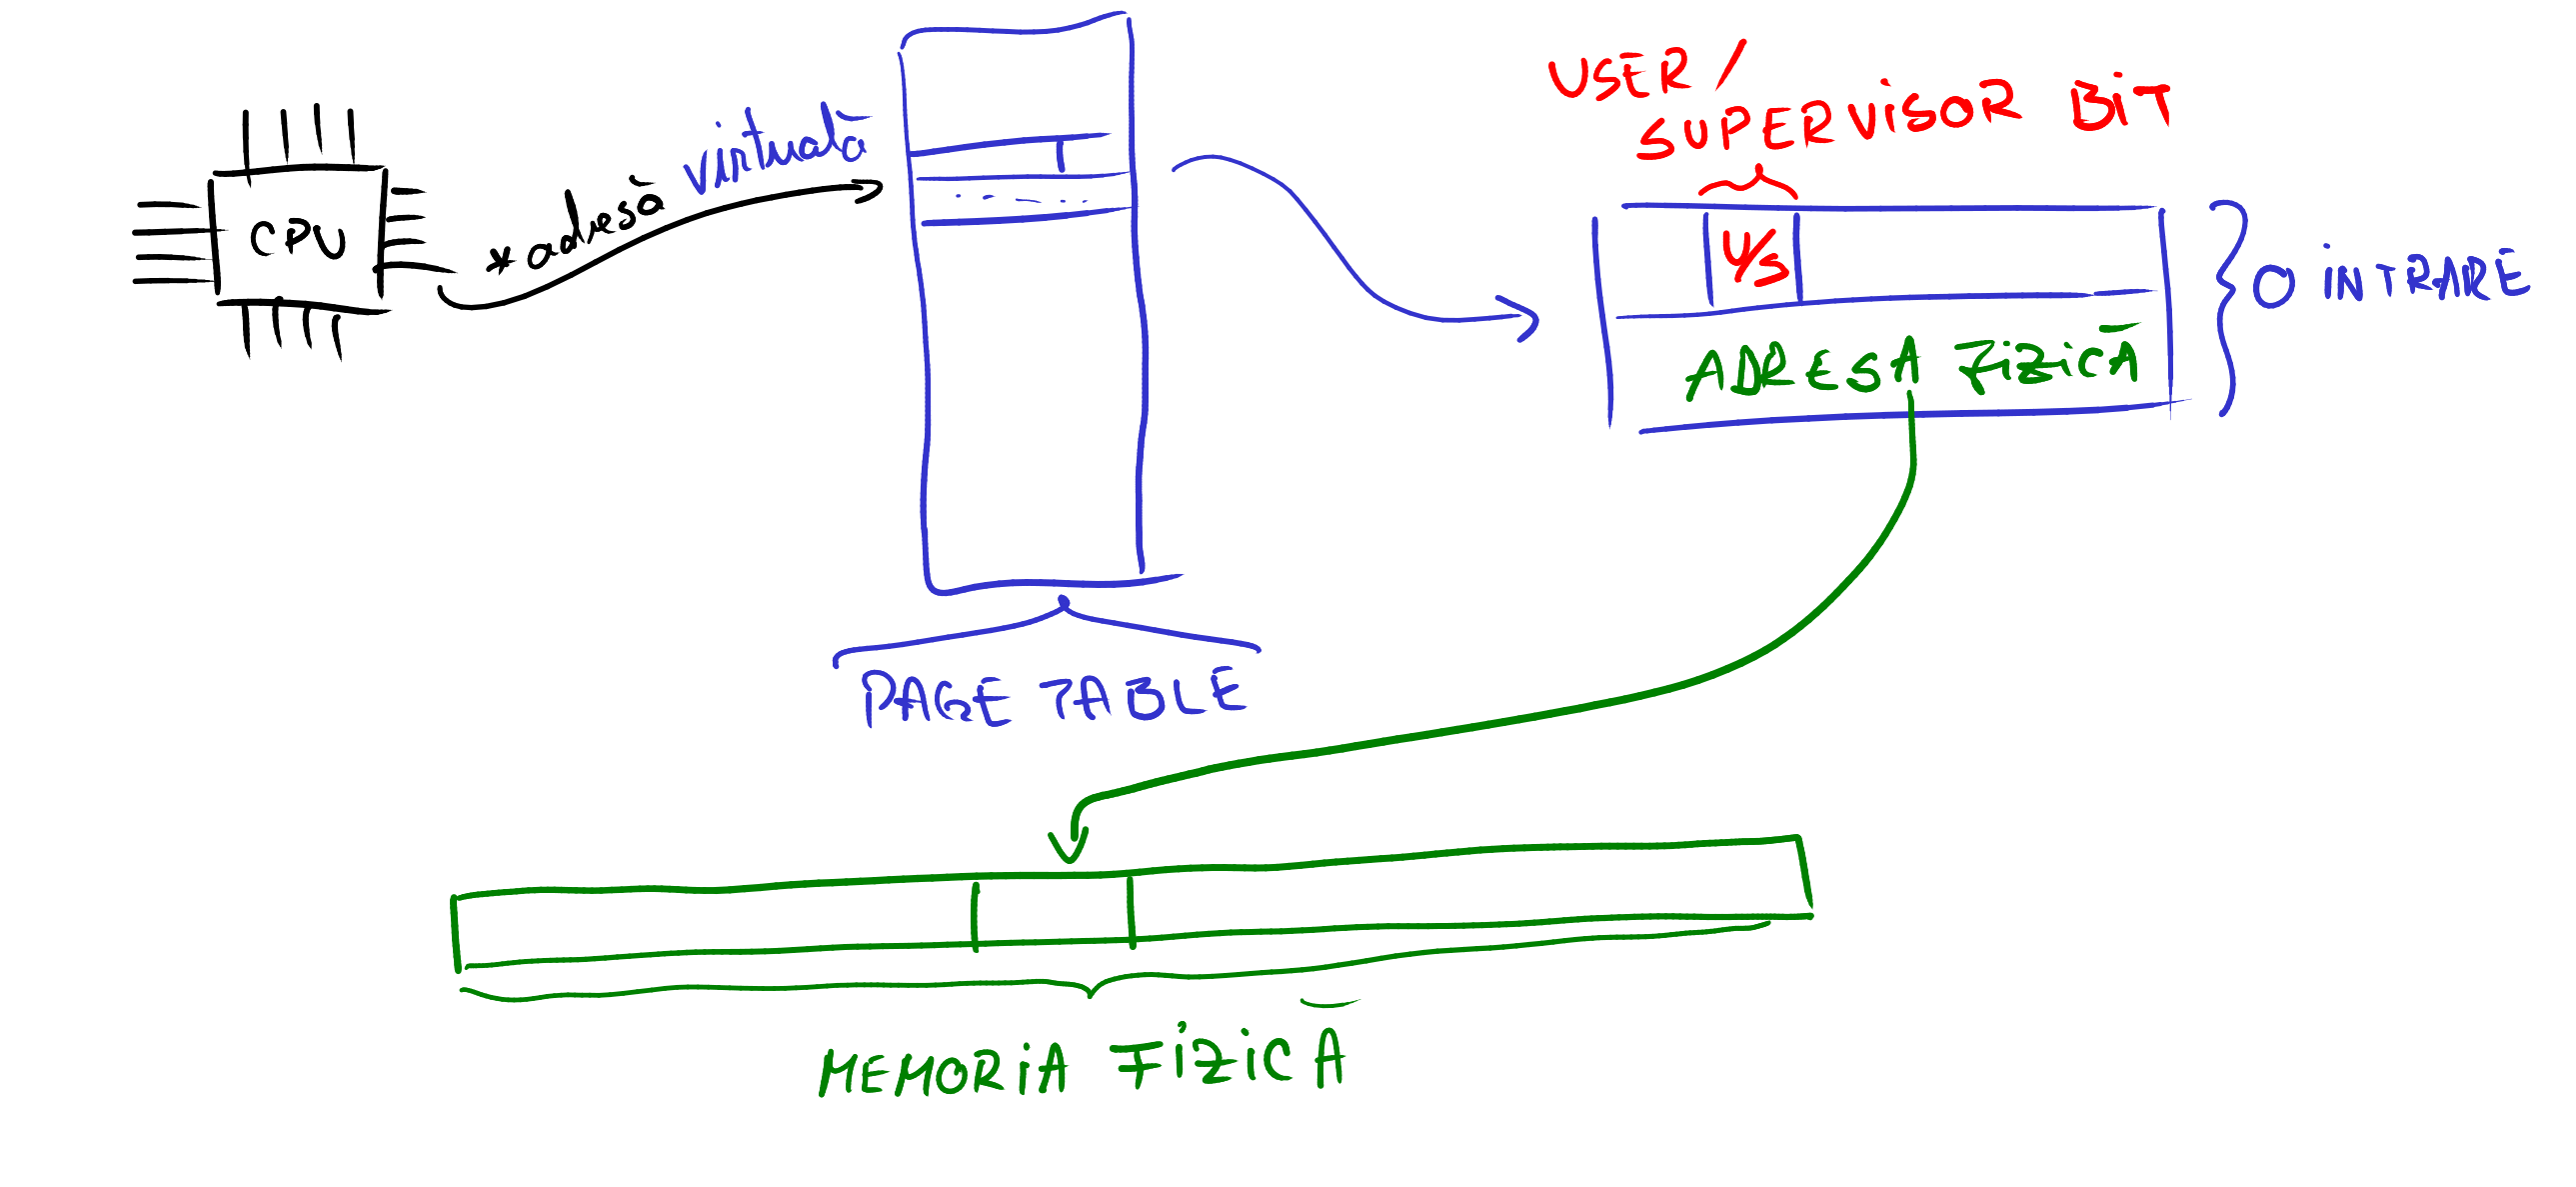
\includegraphics[width=0.9\textwidth]{images/vmem.png}
  \caption{Traducerea adresei virtuale în adresa fizică}
  \label{fig:vmem}
\end{figure}

La momentul descoperirii atacului, întreaga memorie fizică putea fi accesată
prin intermediul kernel-ului, fiind mapată direct în cadrul acestuia. Meltdown
reușește să ignore regulile stricte de separare dintre user și kernel și prin
intermediul acestei legături directe între kernel și restul memoriei poate citi
date fară drepturi asupra acestora. Mitigarea vulnerabilității a constat în
consolidarea mecanismelor de separarea dintre utilizatorul neprivilegiat și
kernel.

\subsection{Exectuarea Instrucțiunilor Tranzitorii}

Scopul atacului este de a accesa și citi date asupra cărora utilizatorul nu are
drepturi, așadar în cadrul atacului vom ținti acest tip de zone de memorie.
După cum am menționat în secțiunea \ref{sec:ooo_exec}, procesoarele moderne
execută adesea instrucțiunile într-o ordine diferită de cea în care apar
acestea în program. Există posibilitatea ca astfel de instrucțiuni să ruleze
înainte ca verificările asupra drepturilor de executare asupra acelei
instrucțiuni să fie finalizate. Să considerăm următoarea secvență de cod:

\begin{lstlisting}[language=c,caption=Executarea instrucțiunilor tranzitorii,
                   escapeinside={(*}{*)}]
   // declararea în prealabil a variabilelor
   int x;
   char kernel_data;

   // accesare kernel produce exceptie
   kernel_data = *kernel_data_addr; (*\label{lst:tranz_deref}*) 
   // instructiunile care urmeaza nu sunt niciodata executate la nivel macro

   // accesarea elementului din tabloul  duce la
   // încarcarea în cache a unei linii care include 
   // index-ul asociat valorii byte-u-lui citit din zona de kernel
   x = probe[kernel_data * 4096]; (*\label{lst:tranz_probe}*)
\end{lstlisting} \label{code:transient}

Se presupune că avem la cunoștință adresa unui secret stocat în zona de kernel
stocată în variabila \texttt{kernel\_data\_addr}. Execuția instrucțiunilor din
linia \ref{lst:tranz_deref} va duce la dereferentia adresei respective, ceea ce va produce un
\emph{Segmentation Fault}. Astfel, la nivel macro, prin intervenția sistemului
de operare, datele de la adresa respectivă nu vor fi accesate, conform
restricțiilor impuse de kernel asupra utilizatorului neprivilegiat.
Comportamentul astfel rezultat al programului este cel așteptat.

La nivel microarhitectural fluxul de execuție diferă. Verificarea drepturilor
de acces asupra unei zone de memorie au loc după accesarea acesteia. Din cauza
\emph{Out-of-Order Execution} și rulării relativ lentă a verificării
drepturilor de accesare, instrucțiunile care succed vor fi executate
speculativ. La nivel microarhitectural datele de la adresa
\texttt{kernel\_data\_addr} vor fi preluate și încărcate în variabila
\texttt{kernel\_data}. Ulterior, tabloul \texttt{probe} vă fi accesat la
index-ul corespunzător \texttt{kernel\_data}, iar pagina corespunzătoare acelei
valori vă fi încărcată în cache (linia \ref{lst:tranz_probe}). Rezultatele obținute vor fi
evident omise când dreptului de acces asupra adresei respective este invalidat,
iar starea registrilor vă trebui resetata la cea anterioara liniei \ref{lst:tranz_deref}. 

Din cauza unui bug în arhitectura majorității procesoarelor, datele încărcate
în cache-ul procesorului în cadrul executării speculative, rămân în cache chiar
și după resetarea stării microarhitecturale. Aceste \emph{Instrucțiuni
Tranzitorii} prin faptul că nu resetează starea cache-ului permit folosirea
tehnicilor specifice atacurilor cache pentru recuperarea secretului
\cite{meltdown2018}.

\subsubsection{Observație - Principiul Localității}\label{sec:locality}

Trebuie făcută o observație importantă pentru linia \ref{lst:tranz_probe}. În cadrul
instrucțiunii tranzitorii pe care vrem să o executăm am accesat tabloul
\texttt{probe} la index-ul $kernal\_data \times 4096$, în loc de
$kernel\_data$. Conform \emph{principiului localității}
\cite{denning2006locality}, când are loc un cache miss procesorul nu încarcă
doar 1 byte din memorie, ci multiplii bytes în funcție de dimensiunea liniilor
din cache (de obicei 64 de bytes). Rezultatul este că în momentul în care un
element \texttt{probe[k]} ar fi accesat, și el și elementele adiacente acestuia
ar fi încărcate în cache. Pentru a putea distinge ușor între elemente adiacente
vom folosi un multiplicator (în acest caz $4096$) mai mare decât dimensiunea 
tipică a unei linii de cache pentru ca accesarea a două elemente adiacente să nu
determine încărcarea în cache a unor blocuri cu zone comune.

\subsection{Gestionarea Excepțiilor}

Pentru a nu întrerupe fluxul de execuție și a putea interpreta datele rezultate
în urma \emph{Instrucțiunilor Tranzitorii} trebuie tratate execeptiile apărute
în mod natural. Conform lucrării de cercetare \cite{meltdown2018} avem două
variante: suprimarea sxcepțiilor și tratarea explicită a excepțiilor.

\subsubsection{Duplicarea Procesului}

O metodă trivială presupune duplicarea (\emph{forking}) procesului chiar înainte
de declanșarea excepției. Linia \ref{lst:tranz_deref} a codului ar fi astfel executata în procesul
copil, care va fi terminat de către sistemul de operarare. Efectele secundare 
apărute în urma execuției speculative pot fi apoi măsurate din procesul părinte
prin intermediul unui canal secundar (\emph{side-channel}), eg. memoria cache.

\subsubsection{Signal Handler}

O metodă alternativă este instalarea unui \emph{signal handler} care se
declanșează la apariția excepției corespunzătoare (eg. \emph{Segmentation Fault})
Astfel evităm terminarea programului de către sistemul de operare și reducând 
timpul de execuție necesar creării unui nou proces.

\subsubsection{Suprimarea Excepțiilor}

Putem de asemenea preveni declanșarea excepțiilor în totalitate. În cadrul
execuției speculative se pot executa instrucțiuni care nu s-ar executa în mod
normal din cauza unei predicții greșite a căii urmate de fluxul de instrucțiuni
în urma unei bifurcări. Astfel, deoarece la nivel macro instrucțiunile ilegale
nu vor fi executate, excepția nu va fi declanșată de sistemul de operare, chiar
dacă la nivel microarhitectural, liniile de cod au fost executate speculativ,
iar efectul secundar a avut loc. Această abordare implică antrenarea oracolului
de prezicere a bifurcărilor (\emph{branch predictor}) și va fi descris în
cadrul discuției despre \emph{Atacuri Spectre} \cite{spectre2019}.

\subsection{Trecerea din planul micro în planul macro}\label{sec:step_receive}

Ca urmare a gestionării excepțiilor, execuția programului continuă
neîntreruptă. În urma executării instrucțiunilor tranzitorii, la nivel
microarhitectural starea sistemului s-a schimbat, prin încărcarea în cache a
adresei accesate speculativ. Prin intermediul tehnicilor specifice atacurilor
asupra memoriei cache (descrise în secțiunea \ref{sec:atacuri_cache}) putem crea un
canal secret de comunicare (covert channel). Va fi prezentată inițial metoda de
transmitere a unui bit pe canalul secret, iar ulterior această metodă va fi
extinsă la transmiterea unui byte.

Pentru a transmite un bit se procedează în felul următor. Pentru transmiterea
de informație se executa o serie de instrucțiuni tranzitorii în urma cărora
zona de memorie dorita este încărcată în cache. Pentru citirea informației de
pe canalul ascuns este folosită tehnica \emph{FLUSH and RELOAD}
(\ref{sec:flush_reload}). Inițial se folosește instrucțiunea \texttt{clflush}
pentru eliberarea din cache (eviction) a adresei tintă, iar apoi se așteaptă
transmiterea unui bit de informație. După trecerea perioadei de timp se măsoară
timpul necesare accesării valorii de la adresa tintă. Dacă timpul de accesare
este mic (sub un prag stabilit anterior) îl clasificăm ca \emph{cache hit}. În
acest caz, constatăm că victima a accesat în fereastra de timp adresa de
memorie prin intermediul unei instrucțiuni tranzitorii, și a transmis atfel un
bit cu valoarea emph{1}. Dacă timpul de accesare este mare (peste pragul
stabilit anterior), clasificăm accesarea că un \emph{cache miss}. În acest caz,
victima nu a executat instrucțiunile tranzitorii corespunzătoare încărcării în
cache a valorii țintă, deci a transmis implicit un bit cu valoare \emph{0}.

Pentru transmiterea a 1 byte de date (dimensiunea corespunzătoare unui caracter
în format ASCII) se va proceda în felul următor. Conform secțiunii de cod din
\ref{code:transient}, pentru fiecare dintre cele 256 de valori posibilie pe
care le poate avea un byte de informație, se accesează o linie separată în
cache în mod speculativ prin intermediul unui set de instrucțiuni tranzitorii.
Pentru reconstruirea informației, atacatorul vă efectua atacul \emph{FLUSH and
RELOAD} pentru fiecare dintre cele 256 de zone posibile din cache. Inițial,
fiecare dintre cele \emph{256} de adrese trebuie eliminate din cache (se
folosește instrucțiunea \texttt{clflush}). În final, index-ul pentru care s-a
obținut un \emph{cache hit} va corespunde valorii byte-ului de informație
transmis prin canalulu secret (vezi figura \ref{fig:flush_reload}). În
particular, pentru array-ul \texttt{probe} se vă rula \emph{FLUSH and RELOAD}
pentru fiecare dintre \texttt{probe[i * 4096]} (cu $0 \leq i \leq 255$). Dacă
se obține un \emph{cache hit} pentru \texttt{probe[k * 4096]} (cu $0 \leq i \leq
255$), atunci pe canal s-a transmis valoarea \emph{k} \cite{meltdown2018}. 

\begin{figure}[ht]
	\centering
	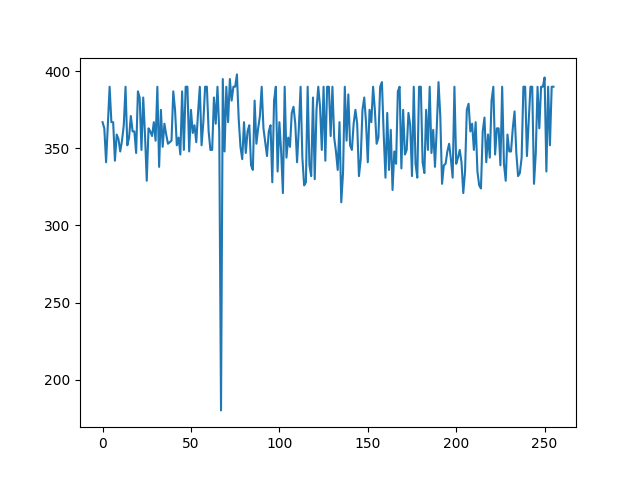
\includegraphics[width=0.9\textwidth]{images/flush_reload_hit.png}
  \caption{Recuperarea unui byte prin Flush \& Reload}
  \label{fig:flush_reload}
\end{figure}

Conform principilui localității (descris aici \ref{sec:locality}) vom mutiplica
valoarea secretului cu \emph{page-size} (în acest caz \emph{4KB}) pentru a
asigura o separare suficient de mare între adresele accesate din
\texttt{probe}. Astfel evităm scenariul în care în urma unei accesări, printre
valorile adiacente indicelui accesat, la un pas, sunt încărcate în cache și
valorile ale unori indici de interes. Astfel, tabloul \texttt{probe} va avea
dimensiunea de exact $256 \times 4096$ pentru pagini de \emph{4KB}.

\subsection{Scenariul și realizarea atacului Meltdown}

La momentul apariției, atacul Meltdown avea ca tintă orice fel de computer
personal, ori mașină virtuală în cloud. Se presupune că atacatorul nu dispune
de acces fizic asupra mașinilor atacate, dar poate executa orice fel de cod în mod
neprivilegiat, cu aceleași drepturi ca un utilzator obișnuit (fără drepturi de
root, ori administrator). Sistemul tintă este protejat de mecanisme considerate
\emph{state-of-the-art} la vremea respectivă (i.e. nu luăm în considerare
mecanismele de protecție apărute ulterior care au ca rezultat mitigarea
atacului, acestea fiind discutate în secțiunea \ref{sec:mitigare_meltdown}),
precum \emph{ASLR} și \emph{KASLR}. Sistemul dispune de asemenea de un
procesor care suportă \emph{Out-of-Order Execution}. Atacul nu se bazează pe
niciun fel de vulnerabilitate de tip software, exploatând doar hibe la nivel
hardware. Astfel, se presupune rularea unui sistem de operare fără probleme
cunoscute care pot fi abuzate pentru elevarea nivelului de privilegii. Ținta
atacatorului va fi orice tip de informație de valoare precum chei de acces,
parole, hash-uri, date personale, etc.

Atacul presupune obținerea adresei din kernel a secretului prin diferite
mecanisme (care nu reprezintă scopul acestei lucrări), ori ghicirea acesteia.
Ulterior se execută pașii descriși mai sus. În primă fază va trebui să se
execute un set de instrucțiuni alese special, care folosesc adresa tintă și se execută
în mod speculativ, devenind ulterior tranzitorii în urma
declanșării unei excepții. Între decodarea adresei virtuale în adresă fizică,
accesarea valorii corespunzătoarea și încărcarea în cache a liniei
aferente \emph{(1)}, și verificarea drepturilor de acces asupra zonei de
memorie conform drepturilor de utilizator și restricțiilor din tabela de
traducere \emph{(2)}, se produce un \emph{race condition}. În cazul în care
\emph{(1)} se execută mai rapid decât \emph{(2)} starea microarhitecturala va
fi modificată în modul dorit, iar abia apoi sistemul de operare va constata
accesul nepermis și va declanșa o excepție. Ajunși în acest punct, rolul
emițătorului este finalizat. Pentru receptarea mesajului se gestionează
excepția de tip \emph{Segmentation Fault} declanșată de sistemul de operare
(printr-una din metodele descrise anterior), iar apoi se folosește \emph{FLUSH
and RELOAD} pentru a recupera secretul (\ref{sec:step_receive}).

Acești trei pași determină obținerea unui byte din secret. Pentru obținerea
întregului secret se iterează prin toate adresele de memorie ale căror valoari
sunt de interes. În mod similar se poate descărca întreaga memorie fizică a 
sistemului tintă.

\section{Sisteme evaluate}

Conform particularităților atacului, orice sistem al cărui hardware este
vulnerabil va fi vulnerabil indiferent de software-ul care rulează (considerând
că patch-ul software nu este aplicat). Într-adevăr s-a constatat că atacul
poate dezvălui informații secrete ale unui utlizator neprivilegiat pe multiple 
sisteme utilizate la scară largă.

\subsection{Linux}

Meltdown a putut fi rulat pe multiple versiuni ale kernel-ului de Linux, de la
2.6.32 la 4.13.0, acestea mapând adresele kernelului în spațiul virtual al
oricărui proces neprivilegiat, bineînțeles cu restricțiile de acces aferente, acestea
fiind implementate corect în tabelele de traducere a adreselor \cite{meltdown2018}.

\subsection{Microsoft Windows}

Meltdown a putut fi rulat pe un sistem cu Windows 10, cu actualizările la zi,
chiar înainte de aplicarea patch-urilor. În ciuda modului diferit în care este
mapată memoria fizică și management-ului diferit al acesteia, majoritatea memoriei
fizice tot se poate citi prin intermediul atacului. Cercetătorii au putut citit 
întregul binar al kernelul-ului de Windows \cite{meltdown2018}.

\subsection{Android}

Deoarece Android-ul are la bază tot Kernel-ul de Linux, succesul atacului pe
această platforma depinde de procesorul instalat pe dispozitiv. Astfel în urma
testelor asupra unui Samsung Galaxy S7 rulând un Linux Kernel cu versiunea
3.18.14, atacul nu a avut succes pe asupra procesorului ARM Cortex A53, dar a
funcționat asupra celor marca Exynos dezvoltate de Samsung.

\subsection{Containere}

Tehnologiile de containerizare care împart între ele același kernel sunt și ele
vulnerabile. Meltdown poate fi rulat cu succes în containere Docker, LXC, sau
OpenVZ și s-a demonstrat că prin intermediul lui se pot extrage informații nu
numai din kernel, dar și din celelalte containere care rulează pe aceeași
mașină fizică. Rezultatul vine din cauză că fiecare container împarte kernel-ul
cu toate celelalte, așadar orice proces va avea încărcat în spațiul său virtual
de memorie întreagă memorie fizică a sistemului, prin intermediul kernel-ului
împărțit cu celelalte containere și procese care rulează pe același sistem.

\subsection{ARM și AMD}

În ciuda succesului pe arhitectura \emph{Intel} și pe câteva modele
\emph{Exynos}, atacul nu a putut fi executat cu succes pe procesoare
\emph{AMD}. \emph{AMD} susțin că acest rezultat se datorează unor diferențe
arhitecturale în comparație cu \emph{Intel} \cite{amd_response}. În cazul
\emph{ARM}, signrul procesor afectat ar fi modelul \emph{Cortex-A75}, conform
\cite{grisenthwaite2018cache}. Deoarece detaliile de implementare ale
microarhitecturilor nu sunt în general dezvăluite publicului larg nu se poate
determină cu exactitate ce a determinat aceste diferențe.

\section{Performanța}

Performanța atacului depinde de modul și eficiența cu care se câștigă
\emph{race condition}-ul. Indiferent de locația din memorie în care se află
datele dorite, s-a demonstrat că \emph{race condition}-ul poate fi câștigat,
dar diferențele de performanță sunt notabile.

\subsection{Secretul în cache}

Când datele sunt în imediata apropiere a procesorului (în cache-ul \emph{L1}),
\emph{race condition}-ul poate fi castigat cu ușurință. Astfel s-au obținut
performanțe ridicate de până la $582$ KB/s cu rata de eroare de până la
$0.003\%$ (Intel Core i7-8700K). O variantă mai lentă a atacului care reduce
eroarea la $0$ ajunge la viteze de $137$ KB/s \cite{meltdown2018}. 

În cazul în care secretul se află în cache-ul \emph{L3}, dar nu în cache-ul
\emph{L1}, \emph{race condition}-ul încă se poate căștiga des, dar viteza vă fi
mult mai mică, de până la $12.4$ KB/s, cu erori de până la $0.02 \%$
\cite{meltdown2018}.

\subsection{Secretul în afara cache-ului}

În acest caz câștigarea \emph{race condition}-ului este mai dificilă. S-au
observat rate de transimitere a datelor de sub $10$ B/s pe majoritatea
sistemelor. Aceste rezultate au putut fi îmbunătățite cu ajutorul a două
optimizări. Acestea presupun preîncărcarea zonelor de memorie din cache prin
intermediul unor thread-uri care rulează în paralel (conform
\cite{gruss2016prefetch}) și abuzând de implementarea cache-ului conform
principiului localitații (vezi \ref{sec:locality}) prin accesarea speculativă a
zonelor adiacente țintei, astfel încărcând în cache și adresa țintă.
Optimizările cresc viteza de citire până la $3.2$ KB/s \cite{meltdown2018}.

\section{Metode de mitigare}
\label{sec:mitigare_meltdown}

\subsection{Hardware}

Meltdown nu exploatează niciun defect de natură software, ci ocolește
restricțiile de acces prezente la nivel hardware prin intermediul 
execuției instrucțiunilor \emph{out-of-order}.

Considerând mecanismele exploatate în cadrul acestui atac, două contramăsuri
posibile ar fi eliminarea completă a \emph{out-of-order execution}, sau
serializarea instrucțiunilor care verifică permisiunile de acces și accesarea
propriu-zisă a zonei de memorie, pentru a evita executarea acestora în paralel.
Aceaste soluții nu ar fi fezabile întrucât impactul pe care l-ar aduce asupra
performanței este mult prea mare.

O soluție mai realistă ar fi separarea la nivel hardware a zonei utilizatorului
și a zonei Kernel printr-un \emph{bit} suplimentar care marchează activarea
acestui sistem. În cazul în care ar fi activat se impune ca adresele kernel-ului
să se regăsească în jumătatea superioară a memoriei, iar adresele
utilizatorului în jumătatea inferioară. Acest mecanism ar avea un impact
neglijabil asupra performanței, deoarece nivelul de permisiuni poate fi dedus
direct în adresa virtuală, astfel dreptul de acces putând fi confirmat sau
infirmat direct, fară accesări suplimentare ale tabelei de traducere.

\subsection{Software -- KAISER}

Deoarece rezolvarea problemelor prezente în hardware-ul aflat în prezent în
folosință este imposibil de implementat în practică, a trebuit găsită o soluție
de natură software. Meltdown poate avea loc deoarece adresele kernel sunt mapate
în spațiul procesului chiar dacă acestea rulează neprivilegiat. Adresele
virtuale mapate sunt legitime și corespund unor adrese fizice. Singurul
mecanism care limitează accesul unui utilizator oarecare în spațiul kernel-ului
constă în restricțiile prezente în tabelele de traducere a adreselor fiecărui
proces. Acest mecanism funcționează la nivel arhitectural, rezultatul final al
execuției fiind cel așteptat. La nivel microarhitectural, s-a demonstrat că
prin intermediul execuției instrucțiunilor într-o altă ordine, în mod
speculativ, se pot accesa din spațiul user-ului zone de memorie din kernel
înainte ca dreptul de acces să fie confirmat. Soluția naturală propusă a fost
utilizarea a două spații de memorie separate pentru fiecare proces: unul
dedicat utilizatorului în care kernel-ul nu este mapat, și unul dedicat
kernel-ului în care spațiul utilizatorului nu este mapat. Din diverse motive de
performanță și practicalitate, printre care faptul că nemaparea spațiului
utilizatorului în Kernel ar presupune rescrierea unor porțiuni considerabile
din Kernel, s-a ajuns la implementarea pe majoritatea sistemelor a unei soluții
bazate pe KAISER (\cite{gruss2017kaslr}) (în Kernel-ul de Linux aceasta poartă
numele de KPTI sau PTI -- \emph{Kernel Page-Table Isolation}).

KAISER a fost propus ca soluție pentru atacurile asupra \emph{Kernel Address
Space Layout Randomization} (KASLR) și presupune o metodă de separare a
spațiului kernel de spațiul utilizatorului. Acest mecanism de protecție are la
bază conceptul de spațiu de adrese fantomă (\emph{shadow address space}).
Astfel, în mod neprivilegiat adresele kernel nu sunt mapate, iar în mod
privilegiat adresele utilizatorului sunt mapate și vegheate de mecanismele de
securitate \emph{SMEP} și \emph{SMAP} care previn execuția codului unui
utilizator în spațiul kernel, sau posibile corupții ale memoriei. Schimbarea
între cele două contexte se face foarte ușor, prin aplicarea unei măști pe biți
asupra registrului \texttt{CR3}, în care se reține adresa tabelei de traducere
corespunzătoare contextului curent. Implementarea acestei soluții previne
atacul Meltdown, întrucât în modul de rulare neprivilegiat nu există adrese
virtuale care să corespunda unor zone sensibile din kernel. S-a demonstrat
că aceasta soluție are costuri de performanță neglijabile, în medie de $0.28\%$
\cite{gruss2017kaslr}.

\begin{figure}[ht]
	\centering
	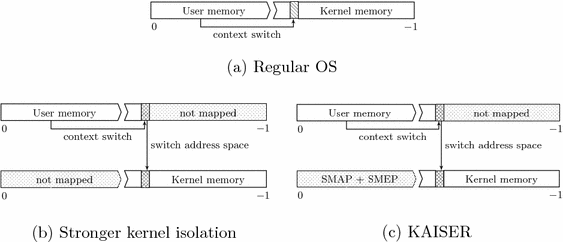
\includegraphics[width=0.9\textwidth]{images/shadowspace.png}
  \caption{Cum se comportă memoria virtuală la schimbarea de context înainte și
      după implementarea KAISER \cite{gruss2017kaslr}}
  \label{fig:shadowspace}
\end{figure}

\section{Reproducerea Atacului}

\subsection{Platforma}

Atacul se poate reproduce cu succes folosind mașina virtuală și ghidul
disponibile pe platforma SEEDLabs \cite{seedlabs_meltdown}. Mediul virtualizat
este important întrucât oferă flexibilitatea rulării sistemului cu un Kernel
învechit care este încă vulnerabil la atacul \emph{Meltdown}. În acest sens se
folosește o mașină virtuală care rulează \emph{Ubuntu 16.04} cu versiunea 4.8.0
cu KPTI neimplementat a Kernel-ului Linux. De asemenea pentru succesul
experimentului este necesară rularea pe o mașină ce are instalat un procesor
marca \emph{Intel} mai vechi de generația a 9-a, deoarece începând cu arhitectura
\emph{Ice Lake} Intel a iceput să introducă patch-uri la nivel de hardware
(\emph{in-silicon}) pentru Meltdown și Spectre.

\subsection{Aspecte importante}

În scopul reproducerii atacului se va crea un scenariu fictiv ce îndeplinește
multiple condiții favorabile montării Meltdown, în scopul evidențierii 
efectelor pe care le poate avea acesta asupra unui sistem. Cunoștințele 
ilustrate astfel nu vor servi decât ca o bază a înțelegerii, și nu ca o unealtă
împotriva unui sistem real.

\subsubsection{Secretul}

Se creează un modul de kernel în interiorul căruia se reține un mesaj secret
cu textul \emph{"Cheia secretă din spațiul kernel"} și adresa acestuia se
afișează în buffer-ul de mesaje dedicat Kernel-ului. Modulul de kernel se
compilează și ulterior se instalează pe sistem, după care se reține adresa
secretului pentru a direcționa atacul exact asupra țintei. În secvența
\ref{lst:kernel_secret_declaration} se observă declararea și afișarea în
buffer-ul de kernel a adresei mesajului secret. În secvența
\ref{lst:kernel_module_install}, se observă instalarea și recuperarea adresei
secretului dorit.

\begin{lstlisting}[language=c, caption=Declararea secretului și afișarea adresei,
                   label=lst:kernel_secret_declaration ]
   static char secret[32] = "Cheia secreta din spatiul kernel";
   /* ... */
   printk("secret data address:%p\n", &secret);      
\end{lstlisting}

\begin{lstlisting}[caption=Instalarea modulului. Aflarea adresei secretului numit "secret",
                   label=lst:kernel_module_install]
   # insmod MeltdownKernelModule.ko
   # dmesg | grep secret
   [21701.143045] secret data address:f8997000
\end{lstlisting}

\subsubsection{Optimizări}
 
Pentru a creste șansele câștigării \emph{race-condition-ului} se iau în calcul toate
cele ce urmează:

\begin{enumerate} \item la fiecare inițiere a atacului se încarcă secretul în cache

   \item succesul atacului depinde de o sincronizare fină la nivel
      microarhitectural, așadar succesul în urma unei singure rulări nu este garantat.
      În practică, pentru aflarea unui byte, atacul asupra aceleiași
      zone de memorie se repetă de multiple ori, iar la urmă se folosesc niște
      tehnici statistice pentru identificarea valorii celei mai probabile
      pentru adresa țintă. Am obținut rezultate bune cu repetări între
      $50$ și $1000$. Un număr mai mic de repetări rezultă în viteze mai mari
      de citire, dar și o rată a erorii mai mare. Un număr mai mare de repetări
      rezultă în viteze mai mici de citire, dar și precizie mai mare.

   \item pragul în funcție de care diferențiem \emph{cache-hituri} de
      \emph{cache-miss}-uri trebuie calibrat. Mai multe detalii în
      secțiunea \ref{subsec:threshold_tool}.

   \item chiar înainte de execuția instrucțiunilor tranzitorii poate fi benefic
      să \emph{"ținem unitățile de calcul ocupate"} prin executarea unor
      instrucțiuni goale. Am evidențiat aceasta idee și în implementarea 
      atacului \emph{Spectre-v1} \ref{code:poc_empty_for}.

   \item declararea statică a unor variabile (keyword \texttt{static}), sau
      accesarea lor în mod repetat poate preveni compilatorul din a optimiza
      fragmentul de cod din care fac parte, ceea ce ar putea determina eșecul
      experimentului. Experimente personale au arătat că acest fapt este foarte
      important în cazul vairabilei \texttt{junk} utilizată la măsurarea
      timpilor de acces în cadrul \emph{FLUSH and RELOAD}
      \ref{code:junk_flush_reload}.

\end{enumerate}

\subsection{Starea actuală - Testarea efectului KPTI}

Sistemul meu principal rulează ultima versiune disponibilă a kernel-ului de
linux în data de 25.05.2022, \texttt{5.17.9-arch1-1}. Am verificat prezența
\emph{KPTI} pe acest sistem cu ajutorul următoarei comenzi,
iar rezultatul a fost pozitiv. 

\begin{lstlisting}[caption=Versiune Kernel și Verifcare prezență KPTI]
   # uname -r
   5.17.9-arch1-1

   # sudo cat /sys/devices/system/cpu/vulnerabilities/meltdown
   Mitigation: PTI
\end{lstlisting}

Într-adevăr, încercarea de a rula aceeași imlementare a atacului Meltdown
pe acest sistem protejat nu duce la niciun rezultat. 

\chapter{Atacuri Spectre}

\emph{Spectre} \cite{spectre2019} este o clasă de atacuri asemănătoare cu
\emph{Meltdown}, care exploatează efectele secundare ale execuției speculative
pentru a extrage informații în mod malițios din spațiul de memorie al unei
victime. La nivel înalt, se bazează pe găsirea sau introducerea unei secvențe
de instrucțiuni în spațiul de adrese al procesului victimă. Mai apoi, execuția
acestei secvențe va crea un canal de comunicare ascuns prin care sunt transmise
date din spațiul de memorie al victimei către atacator. Similar cu
\emph{Meltdown} \cite{meltdown2018}, atacul nu se bazează pe niciun fel de
vulnerabilitate software, ci abuzează vulnerabilități microarhitecturale la
nivel hardware. Chiar dacă în urma executării speculative a unei secvențe de
instrucțiuni, se revine la o stare anterioară, schimbările apărute pe parcus la
nivel de cache pot persista, aceasta fiind vulnerabilitatea principală.

În acest capitol se vor prezenta cele două variante principale din clasa de
atacuri Spectre. În ultimul capitol va fi descrisă o implementare demonstrativă
a variantei 1, care exploatează o zona de memorie partajată cu procesul
victimă.

\section{Diferențe față de Meltdown}

Prima diferență față de \emph{Meltdown} este că variantele \emph{Spectre} evită
provocarea unei excepții prin accesul ilegal al unei zone de memorie. În
schimb, se bazează ori pe antrenarea \emph{branch-predictor-ului} ori pe
injectarea unor adrese alese special în \emph{branch-target-buffer} cu scopul
de a accesa zona de memorie de interes, doar în mod speculativ. Astfel, nu este
necesară gestionarea excepțiilor, atacul interferând minimal, chiar insesizabil,
cu executarea normală a programului.

A doua diferență constă în faptul că \emph{Meltdown} exploatează o
vulnerabilitate specifică procesoarelor \emph{Intel} și câtorva procesoare
\emph{ARM} prin intermediul cărora instrucțiuni executate speculativ pot ignora
restricțiile impuse de bitul \emph{user/supervisor} prezent în intrările din
tabelele de traducere ale adreselor virtuale. Astfel, \emph{Meltdown} poate
accesa memoria Kernel și implicit poate citi toată memoria fizică a sistemului
prin intermediul unui canal ascuns. \emph{Spectre}, în schimb extrage prin
intermediul unei zone de memorie partajată și a unui canal ascuns implementat
în zona respectivă de memorie, doar informații la care victima țintă are acces.
Se încalcă astfel izolarea inter-proces, dar nu se poate accesa direct zona de
Kernel.

Spre deosebire de \emph{Meltdown}, atacurile \emph{Spectre} afectează o plajă
mult mai largă de arhitecturi și s-au dovedit a fi mai dificile de mitigat. Mai
mult, mecanismul care stă la baza mitigarii \emph{Meltdown} (KAISER
\cite{gruss2017kaslr}) nu protejează în niciun fel împotrivă variantelor
\emph{Spectre}.

\section{Spectre V1}
\label{sec:spectrev1}

Varianta întâi de \emph{Spectre} presupune manipularea
\emph{branch-predictor-ului} \ref{sec:branch_prediction} în prezicerea eronată
a ramurii de execuție în cadrul unei structuri decizionale. Astfel, prin
intermediul execuției speculative un atacator poate citi zone arbitrare de
memorie din afara contextului său de execuție, ceea ce încalcă principiile de
izolare impuse de memoria virtuală și sistemul de operare. 

\subsection{Descrierea Atacului}

O secvență de cod precum \ref{code:conditional} se poate regăsi în cadrul unui
apel de funcție (e.g. funcție de sistem sau parte dintr-o bibliotecă), care
primește ca argument o variabilă dintr-o sursă oarecare, neverificată (e.g. în
urma unui apel către un API). Să considerăm situația în care procesul care
rulează codul respectiv (i.e. victima) are acces la un tablou cu elemente de
tip byte \texttt{array} de dimensiune \texttt{array\_size} și la tabloul cu
același tip de elemente, \texttt{probe} de dimensiune $256 * 4096 = 1MB$.
Verificarea de la începutul secvenței de cod are rol în securizarea
programului. În eventualitatea rulării secvenței cu o valoare în \texttt{x} mai
mare sau egală cu \texttt{array\_size} să se evite declanșarea unei excepții
(e.g. \emph{Segmentation Fault}), sau a accesării unei alte zone de memorie din
cadrul de execuție a procesului victimă (e.g. dacă valoarea din x reprezintă
diferența dintre adresa de început a tabloului \texttt{array} și adresa de
început a unui alt tablou \texttt{secret}).

\begin{lstlisting}[language=c, label=code:conditional,
                    caption=Executarea speculativă în structura decizională]
  if (x < array_size) {
    /* prin executarea speculativa putem accesa date din afara
       tabloului array fara declansarea unei exceptii */
    data = probe[array[x] * 4096];
  }
\end{lstlisting}

Se consideră cazul în care \texttt{array\_size} nu este încărcat în cache.
Determinarea ramurii care va fi urmată de fluxul de execuție va fi semnificativ
întârziată din cauza cererii din \emph{DRAM} a valorii variabilei respective,
care precede evaluarea condiției logice. Pentru a nu stagna execuția și a ține
unități de lucru din \emph{CPU} inactive se realizează o presupunere informată ce
vizează ramura pe care urmează să continue execuția, prin intermediul \emph{BPU}
(vezi secțiunea \ref{sec:branch_prediction} și figura
\ref{fig:branch_prediction}). Urmând prezicerea se pot executa speculativ
instrucțiunile ce urmează.

\begin{figure}[ht]
	\centering
	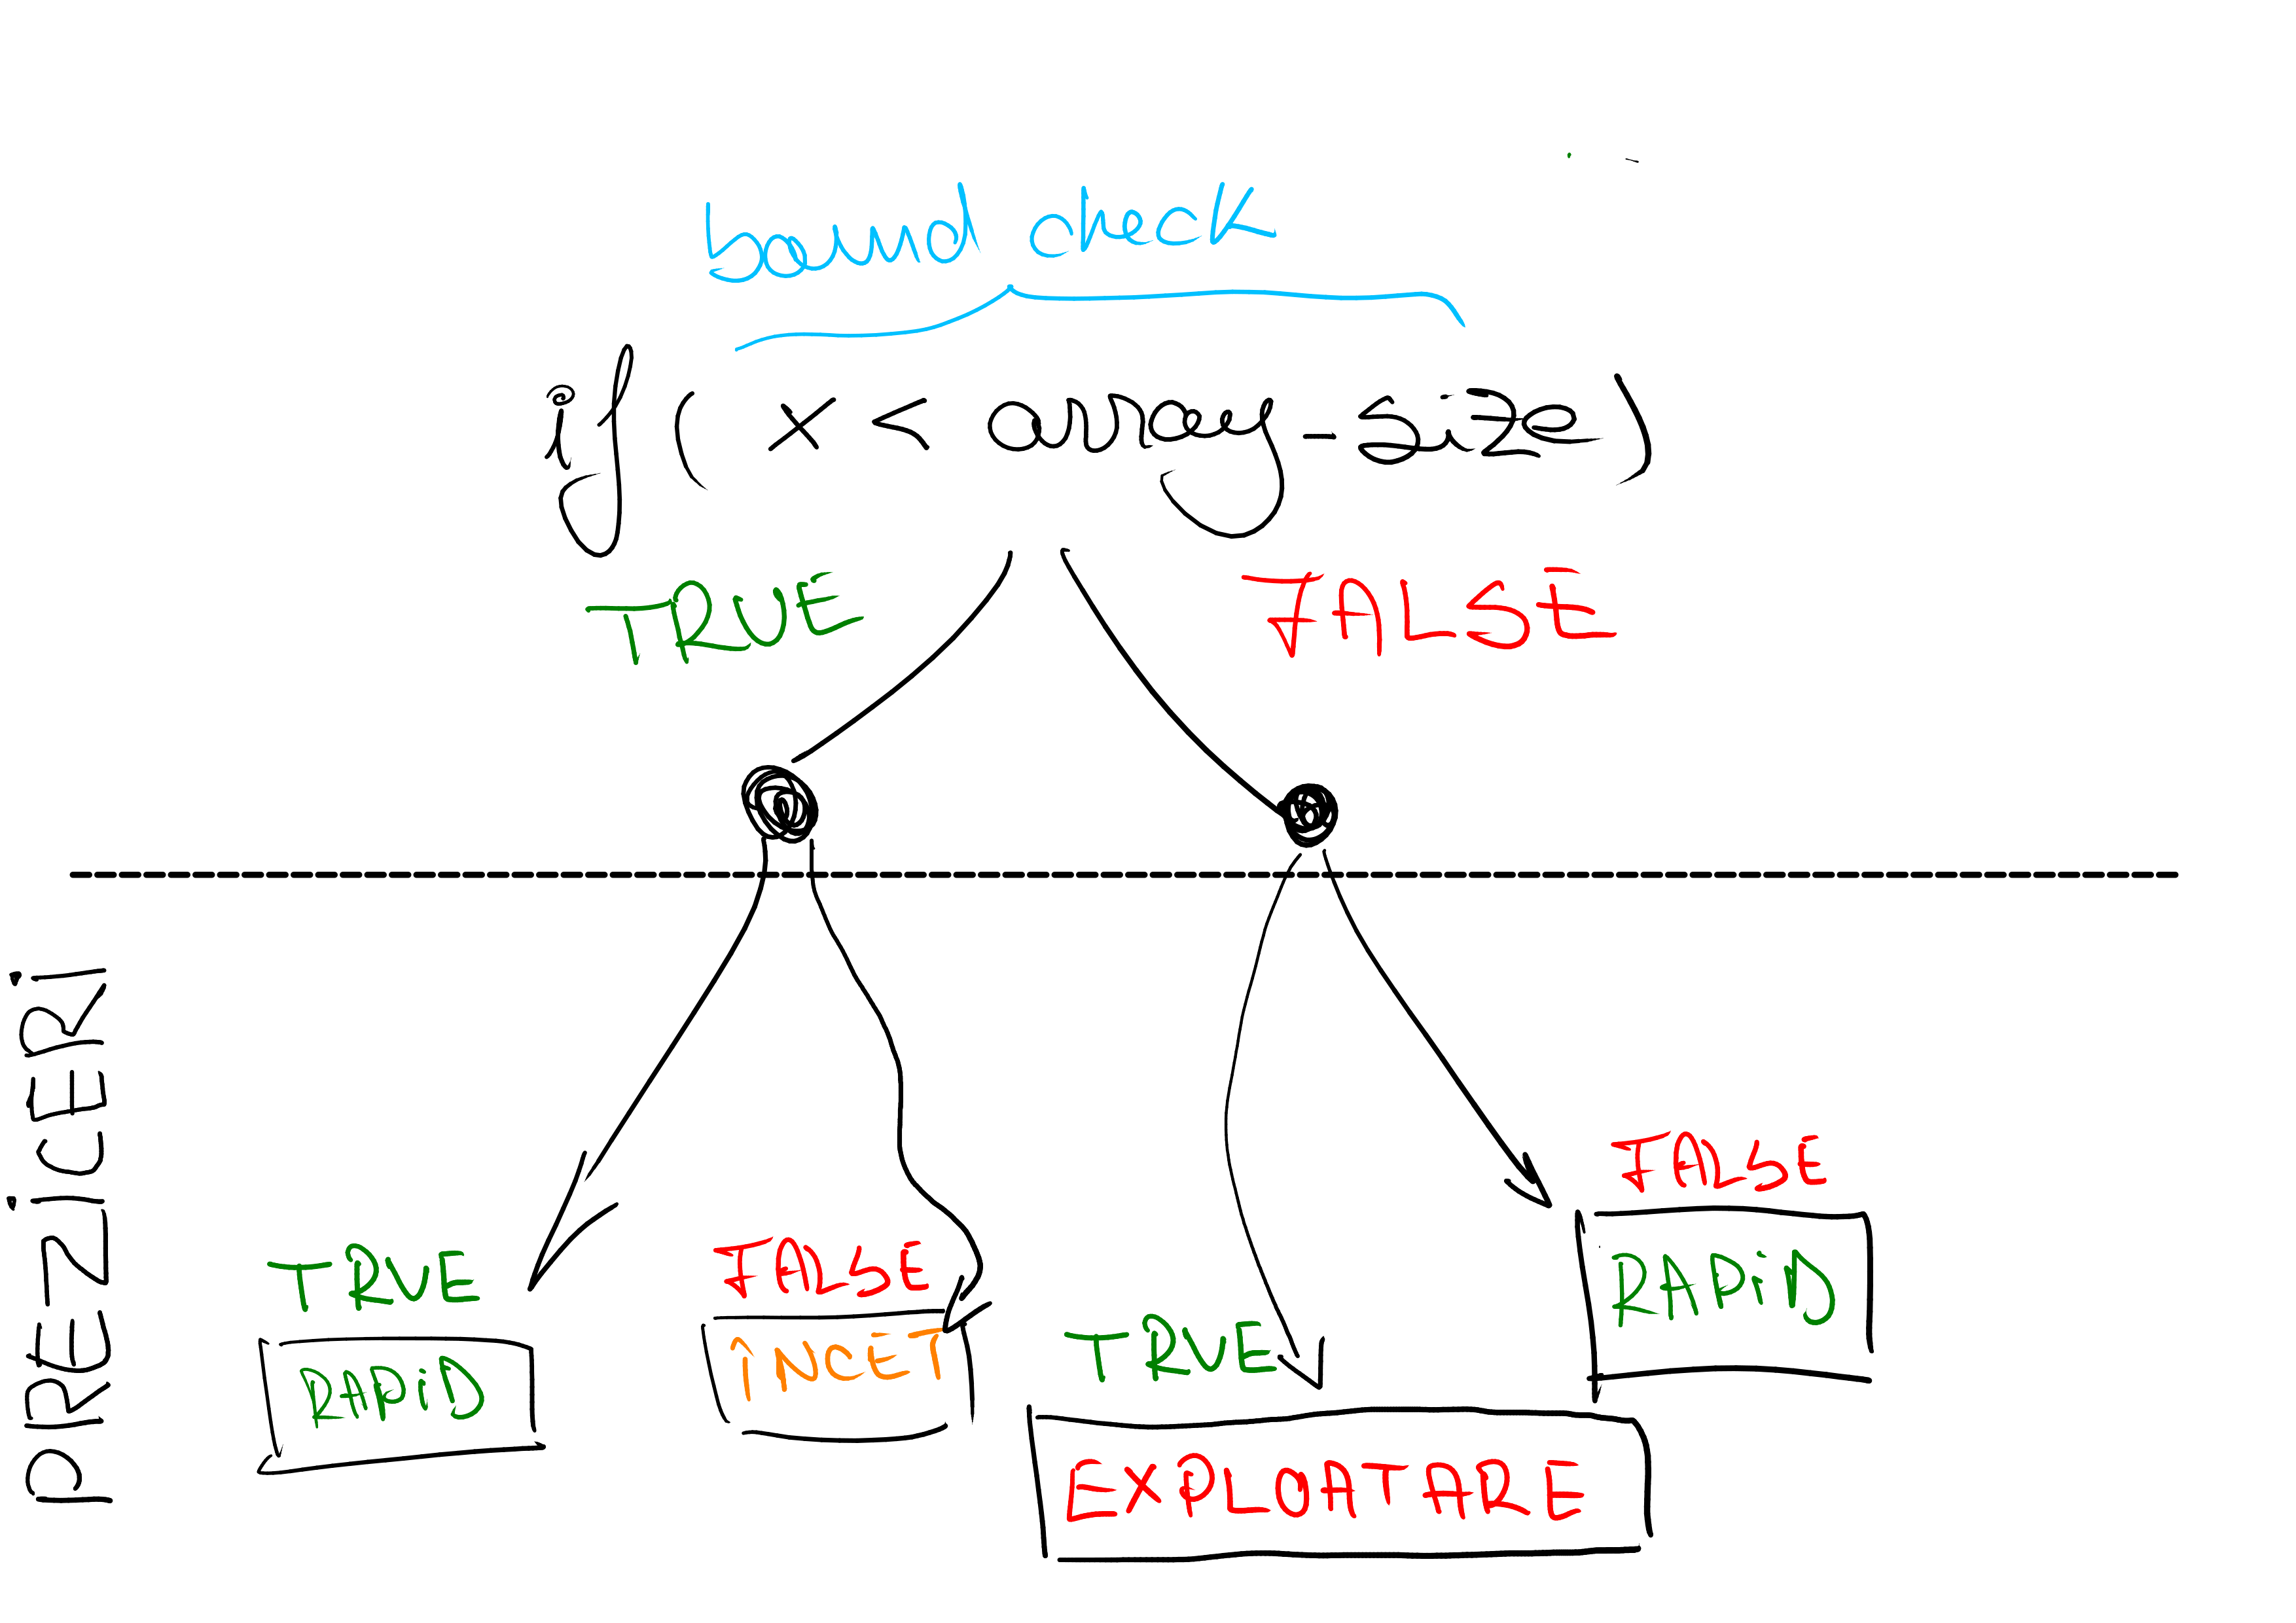
\includegraphics[width=0.9\textwidth]{images/branch_pred.png}
	\caption{Cele patru cazuri posibile în cadrul prezicerii unei ramuri.}
  \label{fig:branch_prediction}
\end{figure}

Acest tipar poate fi exploatat după cum urmează. Un atacator poate executa
intenționat în mod repetat zona respectivă de cod cu valori mai mici decât
\texttt{array\_size}. Astfel, la următoarea execuție a zonei respective,
\emph{BPU} va prezice că fluxul de execuție va urma prima ramură a structurii
decizionale (corespunzătoare evaluării condiției logice la \emph{True}). La
următoarea executarea a zonei respective atacatorul va transmite un \texttt{x}
cu o valoare malițioasă aleasă special în afara limitelor impuse de
\texttt{array\_size} ca în urma evaluării \texttt{array[x]} să întoarcă o
valoare \texttt{k} dintr-o alta zonă din spațiul de memorie al victimei.
Fereastra de timp poate fi suficient de mare ca \emph{linia 4} din
\ref{code:conditional} să fie executată speculativ. Astfel, va ajunge în cache
o linie din memorie corelată cu byte-ul \texttt{k} ce face parte din secretul
accesat speculativ. După ce valoarea din \texttt{array\_size} este primită din
\emph{DRAM}, iar condiția logică este evaluată la \emph{False}, starea CPU-ului
se întoarce la cea dinaintea executării speculative. \emph{Spectre},
exploatează faptul că în urma executării speculative eronate, la nivel
microarhitectural, starea cache-ului din \emph{CPU} nu este resetată.

Pentru finalizarea atacului și recuperarea datelor transmise pe canalul ascuns
se procedează ca în atacul \emph{Meltdown} (vezi \ref{sec:step_receive}). Se
utlizeaza tehnici precum \emph{FLUSH and RELOAD}, sau \emph{EVICT + TIME}
pentru a măsura timpul de acces în fiecare frame de $4KB$ din tabloul
\texttt{probe}. În cazul în care timpul de acces pentru variabila \texttt{k}
este seminificativ mai scăzut comparativ cu al celorlalte adrese, concluzionăm
că byte-ul de date tansmis corespunde cu valoarea \texttt{k} \cite{spectre2019}.

\subsection{Reproducerea atacului}

În practică, urmând strict detaliile descrise anterior, vom obține un nivel
scăzut de acuratețe. Deoarece comportamentul canalului de comunicare ascuns nu
este constant, ci fluctuează și executarea cu succes în mod speculativ a
instrucțiunilor dorite nu este garantată, este necesară repetarea pașilor de
multiple ori pentru fiecare byte, iar apoi determinarea statistică a valorii
celei mai probabile. 

S-a confirmat că această variantă a \emph{Spectre} afectează arhitecturile
\emph{Intel}, \emph{AMD Ryzen} cât și implementări \emph{ARM} care suportă
execuția speculativă. O variantă neoptimizată a atacului implementată în
limbajul \texttt{C} care este prezentată în lucrarea de cercetare
\cite{spectre2019} atinge viteze de $10$ KB/s pe un sistem cu un procesor
\emph{Intel\ i7-4650U}.

\subsubsection{Javascript}

Atacul s-a dovedit practic și în contextul browserelor web. S-a reușit
implementarea acestei variante a \emph{Spectre} în JavaScript și citirea unor
informații private în mod neprivilegiat din spațiul de memorie al procesului în
cadrul căruia rulează codul. Deoarece instrucțiunea \texttt{clflush} nu este
accesibilă prin intermediul limbajului acesta, se folosește o tehnică
alternativă precum \emph{EVICT and RELAOD}. De asemenea instrucțiunea
\texttt{rdtscp} nu este disponibilă, iar motorul din Chrome nu oferă un ceas de
mare precizie pentru a preveni \emph{timing attacks}. Pentru a depăși aceste
obstacole se poate construi un ceas cu precizie suficient de mare prin
incrementarea într-un thread separat a unei zone de memorie controlată de
atacator \cite{spectre2019}.

\subsubsection{Experimente personale}

Dezvoltând ideile anterioare am realizat o implementare personală care
ilustrează un scenariu mai realist în care atacatorul rulează un proces separat
de victimă și împarte cu aceasta doar o zonă de $1$MB de memorie partajată.
Implementarea cât și detaliile se găsesc în capitolul \ref{cap:poc}.

\section{Spectre V2}

Varianta a doua a clasei de atacuri \emph{Spectre} presupune otrăvirea
(\emph{poisoning}) salturilor indirecte (\emph{indirect branches}) (eg. o
instrucțiune de tip \texttt{jump} la o adresă reținută într-un registru). Un
atacator poate astfel determina execuția speculativă a unor instrucțiuni alese
special, prin tehnici care amintesc de ROP (\ref{sec:rop}), pentru accesarea și
apoi extragerea prin intermediul unui canal secret ale unor date accesibile
victimei.

\subsection{Descrierea atacului}

În momentul unui salt indirect, \emph{branch-predictor-ul} va încerca să
prezică adresa la care urmează să se continue execuția pentru a executa
speculativ în avans instrucțiunile ce urmează. În vasta majoritate a cazurilor
se obține o îmbunatățire a timpului de execuție a programului ca urmare a
acestei tehinici, deoarece timpul de recuperare a adresei de destinație poate
fi considerabil în cazul în care adresa de memorie nu este în cache-ul din
\emph{CPU}. Prezicerea se bazează pe istoricul adreselor accesate în trecut în
urma aceluiași salt indirect. Aceste date sunt reținute într-o structură numita
\emph{branch target buffer} și sunt codificate, în funcție de arhitectură, în
funcție de ultimii \texttt{k} biți ai adresei corespunzătoare.

\subsubsection{Antrenarea}

Atacul începe din contextul atacatorului. Acesta mimează salturile indirecte
executate în contextul victimei. Astfel se poate plasa un salt indirect în
contextul atacatorului la aceeași adresă virtuala la care se regăsește saltul
în contextul victimei, sau la o adresă care are în comun ultimii \texttt{k}
biți cu adresa corespunzătoare a victimei. Prin repetarea saltului la o adresă
aleasă de atacator aceasta va ajunge în \emph{branch target buffer}, iar
\emph{branch-predictor-ul} va fi antrenat să prezică că fluxul de execuție va
continua la adresa respectivă. Acest comportament depinde doar de adresa
virtuală și nu ia în considerarea \emph{PID-ul}, adresa fizică, etc. Astfel,
după antrenare, dacă în contextul victimei se execută saltul aferent, se vor
executa speculativ instrucțiuni începând cu adresa injectată de atacator.

S-a observat că atacatorul poate injecta chiar și adrese de memorie la care nu
are acces. Astfel, în contextul său pentru antrenare poate accesa direct adrese
ilegale, iar apoi să gestioneze eventualele excepții declanșate. În acest fel,
atacatorul poate alege orice adresă validă în contextul victimei, chiar dacă
nu are un corespondent valid în contextul său de execuție.

\begin{figure}[ht]
	\centering
	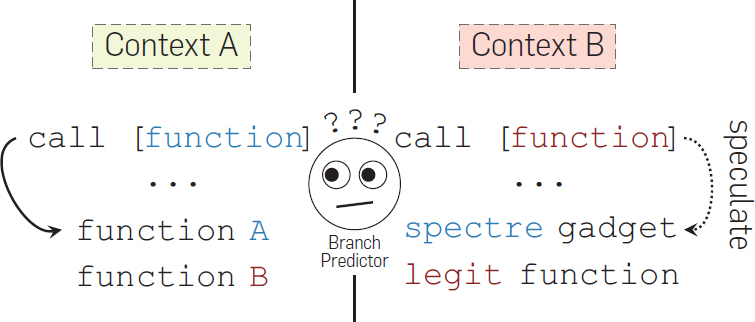
\includegraphics[width=0.9\textwidth]{images/branch_poisoning.jpg}
	\caption{Antrenarea branch-predictorului pentru a executa cod speculativ la 
           adrese alese special de către atacator \cite{spectre2019}.}
  \label{fig:branch_poisoning}
\end{figure}

\subsubsection{Alegerea adresei de destinație}

În urma saltului indirect victima va continua fluxul de execuție la adresa
injectată de atacator. Luând inspirație din atacurile de tip \emph{ROP}
(\ref{sec:rop}) putem alege o zonă de memorie în care începe un așa numit
\emph{Gadget Spectre}. Un \emph{Gadget Spectre} este o secvență de instrucțiuni
a cărei execuție va transmite informații private ale victimei, dorite de
atacator, printr-un canal secret.

Presupunând că victima are acces la doi registri \texttt{R1} și \texttt{R2}, un
gadget suficient ar trebuie să conțină două instrucțiuni după cum urmează.
Prima instrucțiune adună (scade, XOR-ează, înmulțește, etc.) adresa reținută în
registrul \texttt{R1} la registrul \texttt{R2}. A doua instrucțiune accesează
valoarea de la adresa registrului \texttt{R2}. Un atcator va deține în acest
scenariu controlul asupra adresei de memorie accesată (prin intermediul
\texttt{R1}) și asupra modului în care zona de memorie dorită este asociată
la o altă adresă citită prin intermediul \texttt{R2}.

Gadget-urile folosite trebuie să facă parte din zona executabilă din contextul
victimei pentru a garanta execuția speculativă a acestora în \emph{CPU}. 
Gadget-urile pot fi astfel alese din colecția largă de biblioteci partajate la 
care victima are acces, fără a fi nevoie să ne folosim de codul victimei.

\subsection{Rezultate}

În final se obține un atac asemănător conceptual cu \emph{ROP}, dar care exploatează
chiar și cod lipsit de buguri. Gadget-urile rulează doar într-o fereastră 
scurtă de timp și trebuie să transmită informația printr-un canal ascuns pentru
ca aceasta să poată fi recuperată în urma execuției speculative. Multiple teste
au demonstrat că tehnica este eficientă, reușind să injecteze adresa malițioasă în
peste $98\%$ din cazuri în cadrul a milioane de iterații \cite{spectre2019}.

\section{Metode de Mitigare}

De la momentul divulgării acestei clase de atacuri, companiile și cercetătorii
au investit resurse considerabile pentru devoltarea unor metode de mitigare a
vulnerabilităților prezente în sistemele afectate. În această secțiune vor
fi prezentate câteva dintre cele mai relevante metode de mitigare.

\subsection{Software}

\subsubsection{Compilatoare}

În urma unor actualizări pentru principalele compilatoare folosite au fost
introduse multiple opțiuni care vizează mitigarea \emph{Spectre V1}.
Instrucțiunile principale sunt \texttt{-mconditional-branch=all-fix} și
\texttt{-mconditional-branch=pattern-fix} care rezultă intr-o reducere a 
execuției speculative. În urma activării uneia dintre cele doua opțiuni
se realizează o analiză statică a codului pentru identificarea secvențelor 
cu risc înalt. Ulterior sunt introduse în zonele vulnerabile instrucțiuni de 
tip \texttt{LFENCE}, care determină procesorul să aștepte pentru ca toate 
instrucțiunile precedente să fie executate, astfel prevenind potențiale 
instrucțiuni executate speculativ din a modifica starea microarhitecturală.
Ambele optiuni vin cu un cost ridicat de performanță, care poate să fie 
prea ridicat, afectând practicalitatea codului \cite{v1_mitigations}.

Alternativ se pot utliza flag-uri de optimizare precum \texttt{-O0} sau 
\texttt{-O3}, care au ca efect schimbări la nivel de instrucțiuni de asamblare.
Din experimente personale am observat că variantele implementate de mine
ale \emph{Spectre V1} nu întorc niciun rezultat când sunt folosite aceste 
flag-uri de optimizare.

\subsubsection{Retpoline}

\emph{Retpoline} este o secvență specială de cod care transformă un salt 
indirect intr-o instrucțiune de tip \texttt{ret} pentru a garanta că 
\emph{RSB} (\emph{Return Stack Buffer}) este folosit în loc de
\emph{BTB} (\emph{Branch Targe Buffer}). Orice predicție greșită a
adresei dintr-un salt indirect rezultă într-o buclă infinită în 
cadrul execuției speculative. Practic, este eliminată execuția
speculativă pentru salturile indirecte. \emph{AMD} a propus o
implementare alternativă a \emph{Retpoline}, specifică arhitecturii
lor care obține rezultate mai bune \cite{bhi_spectre_2022}. 

Retpoline a dat rezultate bune pe arhitecturile \emph{Intel} și
\emph{AMD}, dar nu și pentru \emph{ARM}.

\subsubsection{ARM}

Pentru arhitecturile mai vechi s-au introdus instrucțiuni care 
pot invalida adresele prezise în \emph{BTB}.

\subsection{Hardware}

\subsubsection{Intel/AMD IBPB}

Reprezintă o barieră care odată introdusă în cod împiedică execuția unui salt
indirect din a influența salturi indirecte ce iau loc după barieră
\cite{intel_mitigations} \cite{amd_mitigations}.

\subsubsection{Intel/AMD STIBP}

Această tehnică împiedică partajarea stării din \emph{Branch Predictor} între
hiper-thread-uri ale aceluiași nucleu \cite{intel_mitigations}
\cite{amd_mitigations}.

\subsubsection{Intel/AMD (e)IBRS}

\emph{Indirect Branch Restricted Speculation} are ca țintă atacurile de tip
\emph{Spectre V2}. Considerând că într-un sistem există 4 nivele de 
privilegii în baza cărora funcționează unitățile de prezicere, această 
soluție încearcă să prevină straturi care rulează cu un nivel scăzut de 
privilegii să influențeze straturi care funcționează la un nivel înalt de
privilegii. Pe noile arhitecturi \emph{ARM} s-au introdus soluții asemănătoare
cu numele \emph{FEAT\_CSV2} \cite{intel_mitigations} \cite{amd_mitigations}.

\section{Starea Actuală}

Principalele tehinici de mitigare folosite în practică la care recurge sistemul
de operare sunt \emph{Retpoline} și \emph{(e)IBRS}. \emph{Retpoline} este
folosit în cazul în care mitigarile la nivel de hardware nu sunt disponibile,
sau în cazul în care impactul asupra performanței este mai ridicat decât în
cazul soluției software. În restul cazurilor sistemul de operare va recurge 
cel mai probabil la utilizarea \emph{IBRS}, sau a soluțiilor similare pe alte
arhitecturi.

În ciuda eforturilor de mitigare, un nou studiu a fost publicat
\cite{bhi_spectre_2022} care demonstrează cum acestea pot fi ocolite,
implementând o varianta puternică a \emph{Spectre V2} numită \emph{Branch
history injection}. Prin intermediul acesteia se pot extrage informații în mod
neprivilegiat din memoria kernel prin intermediul unui program executat în
userland.

\chapter{POC -- Spectre-V1}
\label{cap:poc}

În lucrarea de cercetare în care este prezentată clasa de atacuri spectre și
variații ale acestora \cite{spectre2019}, este pusă la dispoziție și o 
implementare cu scop demonstrativ în care tehnicile descrise sunt utlizate
pentru a citi conținutul unui buffer din spațiul de memorie al procesului
în rulare. Victima și atacatorul sunt combinate astfel într-o singură entitate,
ceea ce rezultă într-un scenariu complet nerealist. În acest capitol voi descrie
o implementare personală și diferită în abordare a atacului, cu scopul de a ilustra
un scenariu mai realist în care această vulnerabilitate poate fi exploatată.

\section{Detalii de implementare}

\subsection{Scenariul}

Considerăm scenariul în care pe un sistem cu actualizările la zi, cu hardware
susceptibil variantei 1 a Spectre (am rulat testele pe computer-ul personal ce
rulează cu un procesor marca \emph{Intel} - generația a 8-a), rulează în mod
privilegiat un proces vulnerabil (\emph{victima}). Victima poate primi cereri
de la alte procese (\emph{clienți}), în urma cărora furnizează un rezultat prin
intermediul unei zone partajate de memorie, separată complet de orice zonă
privată din cadrul spațiului său de memorie. Un client comunică și se sincronizează
cu victima (pentru a evita \emph{race-condition-uri}) prin intermediul unor fișiere
uzuale și a unor fișiere de blocare (\emph{lock files}).

Voi demonstra cum, prin intermediul zonei de memorie partajată, un atacator poate 
obține date private din spațiul de memorie al victimei, folosind tehnici specifice
variantei 1 a clasei de atacuri Spectre \ref{sec:spectrev1}.

\subsection{Vulnerabilitatea}

În cadrul cererilor, atacatorul trimite victimei o mulțime de indici: $\{i_0,
i_1, \dots, i_n\}$. Pentru fiecare indice $i_k$, victima va prelua o valoare dintr-un
tablou static intern, \texttt{array1[i\_k]}. Va realiza apoi o serie de calcule
oarecare, pe baza unei valori din zona partajată cu clienții (\texttt{array2}),
aflată la o poziție proporțională cu \texttt{array1[i\_k]}.

Să considerăm secțiunea următoare de cod:

\begin{lstlisting}[language=c, caption=Secțiune vulnerabila din codul victimei]
unsigned int array1_size = 16;
uint8_t array1[16] = { 1,2,3,4,5,6,7,8,9,10,11,12,13,14,15,16 };

void victim_function(size_t x) {
	static uint8_t temp = 0;  /* declararea statica previne optimizari neprevazute ale compilatorului */
	if (x < array1_size) {
    // calcule cu o valoare din array2 la indice proportional cu array1[x]
    temp &= array2[array1[x] * 512];
	}
}
\end{lstlisting}

Funcția \texttt{victim\_function} este apelată cu fiecare indice $i_k$ primit de
la atacator, transmis prin intemediul parametrului \texttt{x}. Se poate
observa verificarea \texttt{x < array1\_size} ce previne accesarea unor
poziții în afara limitelor tabloului. Astfel, codul poate fi considerat
sigur din punct de vedere software. În schimb, un atacator poate alege 
valorile într-un mod specific ce va determina schimbări la nivelul cache-ului,
măsurabile prin intermediul zonei partajate de memorie, care pot dezvălui 
informații secrete din spațiul victimei.

\subsubsection{Zona partajată}

Zona partajată de memorie este creată de către victimă și încărcată de către
atacator \textbf{doar cu drepturi de citire}, după cum urmează:

\begin{lstlisting}[language=c, caption=Maparea zonei partajate în atacator]
// mapare a zonei partajate în array2 (cache side channel)
int fd = open(shared_memory_name, O_RDONLY);
array2 = (uint8_t*)mmap(NULL, 256 * 512, PROT_READ, MAP_SHARED, fd, 0);
\end{lstlisting}

\subsection{Citirea unui byte}

În cadrul dezvoltării de aplicații, dezvoltatorii folosesc mecanisme de sicronizare și tehnici
specifice \emph{IPC} pentru transmiterea în siguranță și fară pierderi a datelor
de la client la server și invers. În cadrul acestui atac, atacatorul reușește
să citească date de la victimă cu mare precizie datorită utilizării acestor
tehinici.

\subsubsection{Pasul 1 - Preluarea lacătului}

Transmiterea datelor și procesarea acestora de către victimă au loc separat. 
Acest fapt este garantat prin utilizarea unor emph{lock files} \cite{file_locks},
care permit executarea unei secvențe de instrucțiuni numai când procesul în cauză
deține lacătul.

La pasul 1, atacatorul preia lacătul în felul următor:

\begin{lstlisting}[language=c, caption=Preluarea lacătului]
	locked = -1;
	while (locked != 0) {
		fd_lock = open(lock_file_name, O_CREAT);
		locked = flock(fd_lock, LOCK_EX);
	}
\end{lstlisting}

\subsubsection{Pasul 2 - Transmiterea informației}

Atacatorul transmite un set de indici pe care procesul victimă îi va folosi
pentru accesul datelor. Setul este împărțit într-un număr de $4$ runde. Fiecare
antrenare conține $7$ indici ce determină accesări în limitele tabloului
\texttt{array1} ce au ca scop antrenarea \emph{branch-predictor-ului} în
prezicerea primei ramuri și un indice ce produce o accesare \textbf{speculativă}
în afara \texttt{array1} a unei zone dorite de atacator.

\begin{lstlisting}[language=c, caption=Transmiterea datelor]
	f = fopen(index_file_name, "w");
	training_x = tries % array1_size;

	fprintf(f, "%d ", train_rounds * round_length);
	for (i = 0; i < train_rounds; ++i) {
		for (j = 0; j < round_length - 1; ++j) {
			fprintf(f, "%zu ", training_x); // indice de antrenament
		}
		fprintf(f, "%zu ", index); // indice de atac
	}
	fclose(f);
\end{lstlisting}

Alegerea indicelui de antrenament este importantă. Antrenarea în sine vă rezulta
într-un \emph{cache-hit} care corespunde valorii aferente indicelui de antrenare.
Această valoare poate fi determinată în prealabil și apoi ignorată în cadrul
etapei \emph{FLUSH \& RELOAD}.
	
Indicii sunt scriși într-un fișier "index.txt" la care victima are acces. Absența
ulterioară a acestuia va semnifica faptul că victima a terminat procesarea
datelor, fiind folosit de asemenea a un strat suplimentar de sincronizare.

\subsubsection{Pasul 3 - Flush și eliberarea lacătului}

Atacatorul eliberează zona partajată de memorie din cache pentru a putea urmări
schimbările determinate de acțiunile victimei. În final se eliberează lacătul pentru
a permite victimei să proceseze datele transmise.

\begin{lstlisting}[language=c, caption=Flush și eliberarea datelor]
	for (i = 0; i < 256; i++)
		_mm_clflush(&array2[i * 512]);  /* instructiunea clflush */

	// eliberarea lacatului
	unlink(lock_file_name);
	flock(fd_lock, LOCK_UN);
	close(fd_lock);
\end{lstlisting}


\subsubsection{Pasul 4 - Victima preia lacătul}

Asemănător cu atacatorul, pentru a începe executarea instrucțiunilor victima trebuie
să preia accesul asupra lacătului partajat.

\subsubsection{Pasul 5 - Victima procesează indicii primiți}

Victima preia datele transmise de atacator și, pe rând, execută codul vulnerabil cu fiecare
dintre indici. Această serie de instrucțiuni va determina introducerea în cache la un indice
corespunzător cu valoarea secretă a unei valori din zona de memorie partajată \texttt{array2}.

\begin{lstlisting}[language=c, caption=Executarea codului vulnerabil pentru indicii primiți,
									 escapeinside={(*}{*)}]
	for (int i = 0; i < no_items; ++i) {
		_mm_clflush(&array1_size); (*\label{code:poc_flush}*)
		for (volatile int z = 0; z < 100; z++) (*\label{code:poc_empty_for} *)
		victim_function(buffer[i]);
	}

	// stergerea fisierului "index.txt"
	fclose(f);
	remove(index_file_name);
\end{lstlisting}

Este important de menționat că succesul atacului depinde de câțiva factori
ilustrați în secvența de cod de mai sus. În primul rând, absența din cache a
variabilei \texttt{array1\_size} (i.e. linia \ref{code:poc_flush}) este
importantă pentru a facilita câștigarea \emph{race-condition-ului} la nivel
microarhitectural. În al doilea rând, o încărcare ridicată a sistemului rezultă
în acuratețe mai ridicată. Putem simula aceasta încărcare prin executarea unor
instrucțiuni în prealabil (i.e linia \ref{code:poc_empty_for}).

În final, se șterge fișierul cu date "index.txt" și se eliberează
lacătul, pentru a semnala finalul procesării cererii.

\subsubsection{Pasul 6 - Atacatorul finalizează FLUSH \& RELOAD}
\label{subsec:pas6}

Odată cu ștergerea fișierului "index.txt" de către victimă, atacatorul poate
finaliza atacul cu o tehnică specifică atacurilor asupra memoriei cache. În
implementarea de față am folosit tehnica \emph{FLUSH \& RELOAD}.

\begin{lstlisting}[language=c, escapeinside={(*}{*)}]
	addr = &array2[index * 512];
	time1 = __rdtscp(&junk);            /* citeste valoare din cronometru */
	junk = *addr; (*\label{code:junk_flush_reload}*)                      /* acceseaza memoria */
	time2 = __rdtscp(&junk) - time1;    /* calculeaza timpul scurs */
	if (time <= CACHE_HIT_THRESHOLD && index != array1[training_x])
		results[index]++;  /* cache hit - se adauga 1 la scor. */
		/* dupa mai multe repetari indicele cu scor
			 maxim este considerat rezultatul dorit */
\end{lstlisting}

Se măsoară timpul de acces pentru fiecare adresă corespunzătoare fiecăruia dintre
cei $256$ de bytes, iar valorile diferite de cea de antrenament și ai carori timpi
de acces sunt sub un prag stabilit anterior \texttt{CACHE\_HIT\_THRESHOLD} sunt 
marcați într-un tablou de rezultate.

\subsubsection{Citirea datelor secrete}

Repetarea pașilor 1-6 de multiple ori pentru aceeași zonă de memorie este necesară pentru a garanta
acuratețea, iar apoi repetarea și pentru alte zone de memorie rezultă în posibilitatea
citirii întregului spațiu de memorie al victimei.

\section{Rezultate}

Prin rularea procesului victimă în mod privilegiat, se pot citi și reține în
spațiul acestuia date sensibile precum hash-urile parolelor de sistem prezente
în fișierul \texttt{/etc/shadow}. În mod normal aceste date, chiar și încărcate,
sunt în siguranță datorită mecanismelor de separare a contextelor de execuție.
În schimb, în acest scenariu, prin intermediul tehnicilor ilustrate, atacatorul
\textbf{neprivilegiat} poate citi întreg spațiul de memorie al victimei, inclusiv
conținutul fișierului \texttt{/etc/shadow}.

Pentru a evita expunerea unor date sensibile în această lucrarea am ales să rulez atacul asupra unui fișier de configrare. Rezultatele se pot observa în captura de ecran
din figura \ref{fig:spectre_output}.

\begin{figure}[ht]
	\centering
	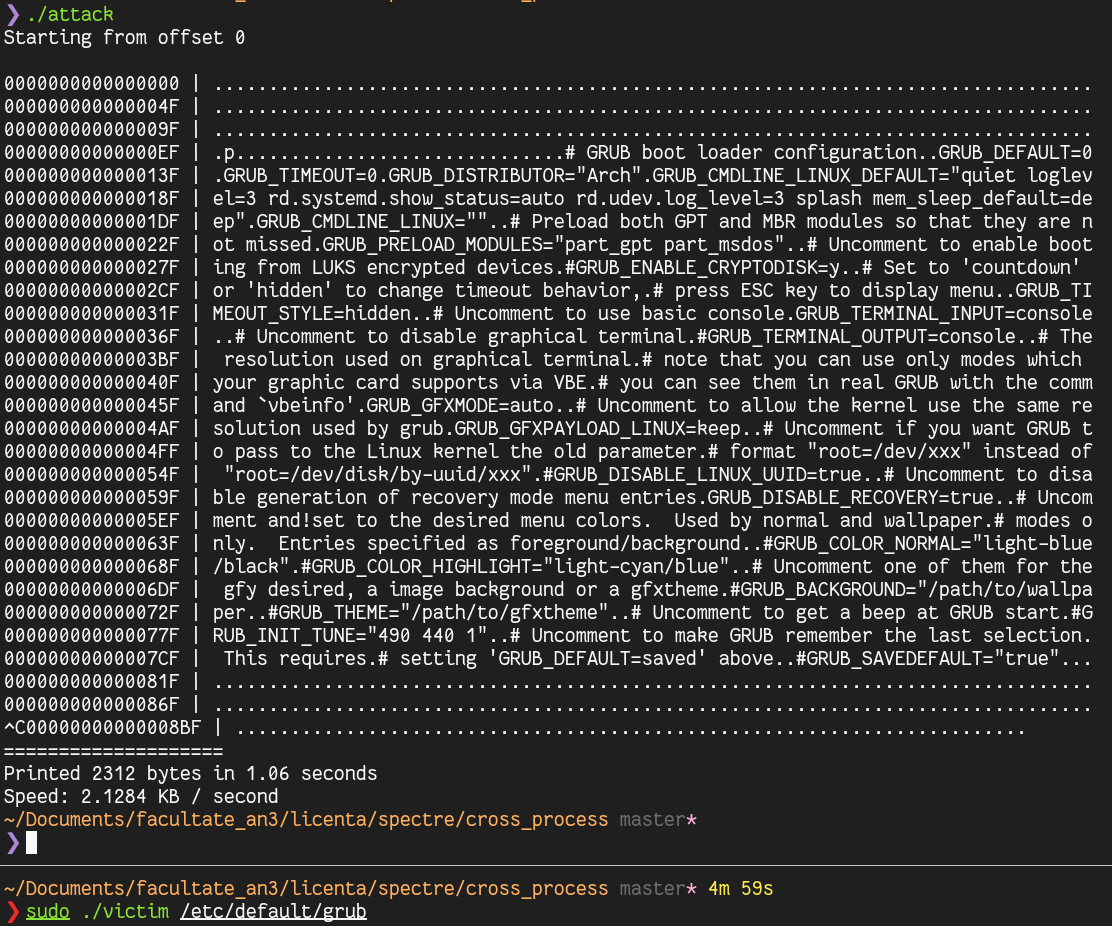
\includegraphics[width=0.9\textwidth]{images/poc_rezultate.png}
	\caption{Configurația bootloader-ului extrasă cu spectre-v1}
\end{figure}
\label{fig:spectre_output}

Am reușit să obțin viteze de citire de până la $2.2$ kB / secundă. Codul
complet poate fi accesat la următoarele adrese:
\href{https://gist.github.com/Stefan-Radu/ca918598c9cce84429f566e020d93d15}{victima} \footnote[1]{accesibil la adresa https://gist.github.com/Stefan-Radu/ca918598c9cce84429f566e020d93d15},
	\href{https://gist.github.com/Stefan-Radu/29732c53a7d552fdec06fb46a801bd51}{atacator} \footnote[2]{accesibil la adresa https://gist.github.com/Stefan-Radu/29732c53a7d552fdec06fb46a801bd51}.


\section{Observații interesante}

Pe parcursul experimentelor am putut face multiple observații și am identificat
diverse elemente care au un rol important în succesul atacului.

\subsection{Pragul pentru determinarea cache-hit-rilor}
\label{subsec:threshold_tool}

Determinarea cache-hit-urilor în toate atacurile și experimentele descrise se
face pe baza unui prag stabilit anterior. Acesta depinde de mulți factori cum
ar fi hardware-ul pe care se rulează codul, și nivelul de încărcare al sistemului.

Pentru utlizarea unui prag cât mai potrivit în cadrul experimentelor am
realizat o unealtă care poate determina cu precizie mare un o valoare
potrivită. Ideea din spatele uneltei este rulearea unuia dintre atacurile
prezentate pe parcursul lucrării cu mai multe valori ale pragului și contorizarea
performantelor obținute. Ulterior, se realizează o medie ponderată a valorilor
obținute în funcție de performanța acestora.

Rulând această unealtă în diverse contexte am observat următorul rezultat
neașteptat. Apar diferențe de până la $20\%$ în cazul în care laptop-ul este 
conectat la o sursă de alimentare în comparație cu cazul în care rulează doar
pe baterie. Explicația ar fi aceea că pentru conservarea energiei când nu este
alimentat extern, se reduce viteza procesorului.

\subsection{Flag-uri de compilare și tipul variabilelor}

În funcție de tipul variabilelor declarate, sau flag-urile de optimizare
utilizate atacul pote rula cu succes, sau eșua total. Spre exemplu, utilizarea
unui tip de date non-static pentru variabila \texttt{junk} în cadrul
\emph{FLUSH \& RELOAD} (secțiunea \ref{subsec:pas6} linia
\ref{code:junk_flush_reload}) poate rezulta în eșecul atacului. Acest eșec
poate, în schimb, fi prevenit prin compilarea fie cu o versiune mai veche a
compilatorului (am testat cu gcc 5.3 care probabil aborda optimizările
diferit), sau cu un flag de compilare explicit (am avut succes cu \texttt{-O},
sau \texttt{-O1}).

\chapter{Concluzii și Direcții Viitoare}

În această lucrare am abordat subiectul \emph{Atacurilor Speculative}. Am
prezentat detalile atacului \emph{Meltdown} care permitea unui utilizator
neprivilegiat citirea oricărei zone din memoria fizică prin intermediul
Kernelului, soluția care a dus la mitigarea acestuia (\emph{KAISER}), cât
și observații personale legate de reproducere. Ulterior am prezentat clasa
de atacuri \emph{Spectre} care permite citirea zonelor de memorie 
accesibile unui proces victimă cu care un proces atacator are în comun
o zonă limitată de memorie. Prezint de asemenea și soluții care au încercat
să mitigheze cu grade variate de succes aceste vulnerabilități. În final,
prezint o implementare inter-proces, cu scop didactic a \emph{Spectre v1}.

Noua variantă a \emph{Spectre} (\emph{BHI}) publicată la începutul anului 2022
demonstrează ineficiența solutilor implementate până în prezent importriva
\emph{Spectre V2}. Astfel, \emph{Spectre} rămâne un subiect deschis de
cercetare. Se pot dezvolta în continuare noi variante ale atacului care pot fi
eficiente chiar și împotriva mitigarilor ce vor apărea în viitorul apropiat. Se
pot dezvolta noi mitigari care să afecteze performanța programelor într-un mod
minimal, mai puțin decât cele deja existente care reduc performanța
considerabil. Se pot evalua implicările atacului pe platforme mai puțin
documentate.

În viitor, îmi doresc să studiez mai în detaliu \emph{Spectre V2} și ulterior,
noua variantă \emph{Spectre BHI} apărută recent, pentru a înțelege mai bine
mecanismele din spate care fac posibile rezultatele obținute. Noile cunoștinte
dobândite, m-ar ajuta în contiuarea cercetării atacurilor speculative.

 
\printbibliography[heading=bibintoc]

\end{document}
